\documentclass[11pt]{article}

    \usepackage[breakable]{tcolorbox}
    \usepackage{parskip} % Stop auto-indenting (to mimic markdown behaviour)
    
    \usepackage{iftex}
    \ifPDFTeX
    	\usepackage[T1]{fontenc}
    	\usepackage{mathpazo}
    \else
    	\usepackage{fontspec}
    \fi

    % Basic figure setup, for now with no caption control since it's done
    % automatically by Pandoc (which extracts ![](path) syntax from Markdown).
    \usepackage{graphicx}
    % Maintain compatibility with old templates. Remove in nbconvert 6.0
    \let\Oldincludegraphics\includegraphics
    % Ensure that by default, figures have no caption (until we provide a
    % proper Figure object with a Caption API and a way to capture that
    % in the conversion process - todo).
    \usepackage{caption}
    \DeclareCaptionFormat{nocaption}{}
    \captionsetup{format=nocaption,aboveskip=0pt,belowskip=0pt}

    \usepackage[Export]{adjustbox} % Used to constrain images to a maximum size
    \adjustboxset{max size={0.9\linewidth}{0.9\paperheight}}
    \usepackage{float}
    \floatplacement{figure}{H} % forces figures to be placed at the correct location
    \usepackage{xcolor} % Allow colors to be defined
    \usepackage{enumerate} % Needed for markdown enumerations to work
    \usepackage{geometry} % Used to adjust the document margins
    \usepackage{amsmath} % Equations
    \usepackage{amssymb} % Equations
    \usepackage{textcomp} % defines textquotesingle
    % Hack from http://tex.stackexchange.com/a/47451/13684:
    \AtBeginDocument{%
        \def\PYZsq{\textquotesingle}% Upright quotes in Pygmentized code
    }
    \usepackage{upquote} % Upright quotes for verbatim code
    \usepackage{eurosym} % defines \euro
    \usepackage[mathletters]{ucs} % Extended unicode (utf-8) support
    \usepackage{fancyvrb} % verbatim replacement that allows latex
    \usepackage{grffile} % extends the file name processing of package graphics 
                         % to support a larger range
    \makeatletter % fix for grffile with XeLaTeX
    \def\Gread@@xetex#1{%
      \IfFileExists{"\Gin@base".bb}%
      {\Gread@eps{\Gin@base.bb}}%
      {\Gread@@xetex@aux#1}%
    }
    \makeatother

    % The hyperref package gives us a pdf with properly built
    % internal navigation ('pdf bookmarks' for the table of contents,
    % internal cross-reference links, web links for URLs, etc.)
    \usepackage{hyperref}
    % The default LaTeX title has an obnoxious amount of whitespace. By default,
    % titling removes some of it. It also provides customization options.
    \usepackage{titling}
    \usepackage{longtable} % longtable support required by pandoc >1.10
    \usepackage{booktabs}  % table support for pandoc > 1.12.2
    \usepackage[inline]{enumitem} % IRkernel/repr support (it uses the enumerate* environment)
    \usepackage[normalem]{ulem} % ulem is needed to support strikethroughs (\sout)
                                % normalem makes italics be italics, not underlines
    \usepackage{mathrsfs}
    

    
    % Colors for the hyperref package
    \definecolor{urlcolor}{rgb}{0,.145,.698}
    \definecolor{linkcolor}{rgb}{.71,0.21,0.01}
    \definecolor{citecolor}{rgb}{.12,.54,.11}

    % ANSI colors
    \definecolor{ansi-black}{HTML}{3E424D}
    \definecolor{ansi-black-intense}{HTML}{282C36}
    \definecolor{ansi-red}{HTML}{E75C58}
    \definecolor{ansi-red-intense}{HTML}{B22B31}
    \definecolor{ansi-green}{HTML}{00A250}
    \definecolor{ansi-green-intense}{HTML}{007427}
    \definecolor{ansi-yellow}{HTML}{DDB62B}
    \definecolor{ansi-yellow-intense}{HTML}{B27D12}
    \definecolor{ansi-blue}{HTML}{208FFB}
    \definecolor{ansi-blue-intense}{HTML}{0065CA}
    \definecolor{ansi-magenta}{HTML}{D160C4}
    \definecolor{ansi-magenta-intense}{HTML}{A03196}
    \definecolor{ansi-cyan}{HTML}{60C6C8}
    \definecolor{ansi-cyan-intense}{HTML}{258F8F}
    \definecolor{ansi-white}{HTML}{C5C1B4}
    \definecolor{ansi-white-intense}{HTML}{A1A6B2}
    \definecolor{ansi-default-inverse-fg}{HTML}{FFFFFF}
    \definecolor{ansi-default-inverse-bg}{HTML}{000000}

    % commands and environments needed by pandoc snippets
    % extracted from the output of `pandoc -s`
    \providecommand{\tightlist}{%
      \setlength{\itemsep}{0pt}\setlength{\parskip}{0pt}}
    \DefineVerbatimEnvironment{Highlighting}{Verbatim}{commandchars=\\\{\}}
    % Add ',fontsize=\small' for more characters per line
    \newenvironment{Shaded}{}{}
    \newcommand{\KeywordTok}[1]{\textcolor[rgb]{0.00,0.44,0.13}{\textbf{{#1}}}}
    \newcommand{\DataTypeTok}[1]{\textcolor[rgb]{0.56,0.13,0.00}{{#1}}}
    \newcommand{\DecValTok}[1]{\textcolor[rgb]{0.25,0.63,0.44}{{#1}}}
    \newcommand{\BaseNTok}[1]{\textcolor[rgb]{0.25,0.63,0.44}{{#1}}}
    \newcommand{\FloatTok}[1]{\textcolor[rgb]{0.25,0.63,0.44}{{#1}}}
    \newcommand{\CharTok}[1]{\textcolor[rgb]{0.25,0.44,0.63}{{#1}}}
    \newcommand{\StringTok}[1]{\textcolor[rgb]{0.25,0.44,0.63}{{#1}}}
    \newcommand{\CommentTok}[1]{\textcolor[rgb]{0.38,0.63,0.69}{\textit{{#1}}}}
    \newcommand{\OtherTok}[1]{\textcolor[rgb]{0.00,0.44,0.13}{{#1}}}
    \newcommand{\AlertTok}[1]{\textcolor[rgb]{1.00,0.00,0.00}{\textbf{{#1}}}}
    \newcommand{\FunctionTok}[1]{\textcolor[rgb]{0.02,0.16,0.49}{{#1}}}
    \newcommand{\RegionMarkerTok}[1]{{#1}}
    \newcommand{\ErrorTok}[1]{\textcolor[rgb]{1.00,0.00,0.00}{\textbf{{#1}}}}
    \newcommand{\NormalTok}[1]{{#1}}
    
    % Additional commands for more recent versions of Pandoc
    \newcommand{\ConstantTok}[1]{\textcolor[rgb]{0.53,0.00,0.00}{{#1}}}
    \newcommand{\SpecialCharTok}[1]{\textcolor[rgb]{0.25,0.44,0.63}{{#1}}}
    \newcommand{\VerbatimStringTok}[1]{\textcolor[rgb]{0.25,0.44,0.63}{{#1}}}
    \newcommand{\SpecialStringTok}[1]{\textcolor[rgb]{0.73,0.40,0.53}{{#1}}}
    \newcommand{\ImportTok}[1]{{#1}}
    \newcommand{\DocumentationTok}[1]{\textcolor[rgb]{0.73,0.13,0.13}{\textit{{#1}}}}
    \newcommand{\AnnotationTok}[1]{\textcolor[rgb]{0.38,0.63,0.69}{\textbf{\textit{{#1}}}}}
    \newcommand{\CommentVarTok}[1]{\textcolor[rgb]{0.38,0.63,0.69}{\textbf{\textit{{#1}}}}}
    \newcommand{\VariableTok}[1]{\textcolor[rgb]{0.10,0.09,0.49}{{#1}}}
    \newcommand{\ControlFlowTok}[1]{\textcolor[rgb]{0.00,0.44,0.13}{\textbf{{#1}}}}
    \newcommand{\OperatorTok}[1]{\textcolor[rgb]{0.40,0.40,0.40}{{#1}}}
    \newcommand{\BuiltInTok}[1]{{#1}}
    \newcommand{\ExtensionTok}[1]{{#1}}
    \newcommand{\PreprocessorTok}[1]{\textcolor[rgb]{0.74,0.48,0.00}{{#1}}}
    \newcommand{\AttributeTok}[1]{\textcolor[rgb]{0.49,0.56,0.16}{{#1}}}
    \newcommand{\InformationTok}[1]{\textcolor[rgb]{0.38,0.63,0.69}{\textbf{\textit{{#1}}}}}
    \newcommand{\WarningTok}[1]{\textcolor[rgb]{0.38,0.63,0.69}{\textbf{\textit{{#1}}}}}
    
    
    % Define a nice break command that doesn't care if a line doesn't already
    % exist.
    \def\br{\hspace*{\fill} \\* }
    % Math Jax compatibility definitions
    \def\gt{>}
    \def\lt{<}
    \let\Oldtex\TeX
    \let\Oldlatex\LaTeX
    \renewcommand{\TeX}{\textrm{\Oldtex}}
    \renewcommand{\LaTeX}{\textrm{\Oldlatex}}
    % Document parameters
    % Document title
    
\title{%
 \line(1,0){430}\\
 MGU - hyper-parameter self-learning using Multi Gated Units in deep neural graphs \\
  \large Experimental Protocol for XCS229ii Winter 2020 \\
  \line(1,0){430}  
  }

    
\date{December 6, 2020}

    
\author{
Andrei Damian \\ Lummetry.AI \\ email: \href{mailto:andrei.damian@lummetry.ai}{andrei.damian@lummetry.ai}
\and
Laurentiu Piciu \\ Lummetry.AI \\ email: \href{mailto:laurentiu.piciu@lummetry.ai}{laurentiu.piciu@lummetry.ai}
}

    
% Pygments definitions
\makeatletter
\def\PY@reset{\let\PY@it=\relax \let\PY@bf=\relax%
    \let\PY@ul=\relax \let\PY@tc=\relax%
    \let\PY@bc=\relax \let\PY@ff=\relax}
\def\PY@tok#1{\csname PY@tok@#1\endcsname}
\def\PY@toks#1+{\ifx\relax#1\empty\else%
    \PY@tok{#1}\expandafter\PY@toks\fi}
\def\PY@do#1{\PY@bc{\PY@tc{\PY@ul{%
    \PY@it{\PY@bf{\PY@ff{#1}}}}}}}
\def\PY#1#2{\PY@reset\PY@toks#1+\relax+\PY@do{#2}}

\expandafter\def\csname PY@tok@w\endcsname{\def\PY@tc##1{\textcolor[rgb]{0.73,0.73,0.73}{##1}}}
\expandafter\def\csname PY@tok@c\endcsname{\let\PY@it=\textit\def\PY@tc##1{\textcolor[rgb]{0.25,0.50,0.50}{##1}}}
\expandafter\def\csname PY@tok@cp\endcsname{\def\PY@tc##1{\textcolor[rgb]{0.74,0.48,0.00}{##1}}}
\expandafter\def\csname PY@tok@k\endcsname{\let\PY@bf=\textbf\def\PY@tc##1{\textcolor[rgb]{0.00,0.50,0.00}{##1}}}
\expandafter\def\csname PY@tok@kp\endcsname{\def\PY@tc##1{\textcolor[rgb]{0.00,0.50,0.00}{##1}}}
\expandafter\def\csname PY@tok@kt\endcsname{\def\PY@tc##1{\textcolor[rgb]{0.69,0.00,0.25}{##1}}}
\expandafter\def\csname PY@tok@o\endcsname{\def\PY@tc##1{\textcolor[rgb]{0.40,0.40,0.40}{##1}}}
\expandafter\def\csname PY@tok@ow\endcsname{\let\PY@bf=\textbf\def\PY@tc##1{\textcolor[rgb]{0.67,0.13,1.00}{##1}}}
\expandafter\def\csname PY@tok@nb\endcsname{\def\PY@tc##1{\textcolor[rgb]{0.00,0.50,0.00}{##1}}}
\expandafter\def\csname PY@tok@nf\endcsname{\def\PY@tc##1{\textcolor[rgb]{0.00,0.00,1.00}{##1}}}
\expandafter\def\csname PY@tok@nc\endcsname{\let\PY@bf=\textbf\def\PY@tc##1{\textcolor[rgb]{0.00,0.00,1.00}{##1}}}
\expandafter\def\csname PY@tok@nn\endcsname{\let\PY@bf=\textbf\def\PY@tc##1{\textcolor[rgb]{0.00,0.00,1.00}{##1}}}
\expandafter\def\csname PY@tok@ne\endcsname{\let\PY@bf=\textbf\def\PY@tc##1{\textcolor[rgb]{0.82,0.25,0.23}{##1}}}
\expandafter\def\csname PY@tok@nv\endcsname{\def\PY@tc##1{\textcolor[rgb]{0.10,0.09,0.49}{##1}}}
\expandafter\def\csname PY@tok@no\endcsname{\def\PY@tc##1{\textcolor[rgb]{0.53,0.00,0.00}{##1}}}
\expandafter\def\csname PY@tok@nl\endcsname{\def\PY@tc##1{\textcolor[rgb]{0.63,0.63,0.00}{##1}}}
\expandafter\def\csname PY@tok@ni\endcsname{\let\PY@bf=\textbf\def\PY@tc##1{\textcolor[rgb]{0.60,0.60,0.60}{##1}}}
\expandafter\def\csname PY@tok@na\endcsname{\def\PY@tc##1{\textcolor[rgb]{0.49,0.56,0.16}{##1}}}
\expandafter\def\csname PY@tok@nt\endcsname{\let\PY@bf=\textbf\def\PY@tc##1{\textcolor[rgb]{0.00,0.50,0.00}{##1}}}
\expandafter\def\csname PY@tok@nd\endcsname{\def\PY@tc##1{\textcolor[rgb]{0.67,0.13,1.00}{##1}}}
\expandafter\def\csname PY@tok@s\endcsname{\def\PY@tc##1{\textcolor[rgb]{0.73,0.13,0.13}{##1}}}
\expandafter\def\csname PY@tok@sd\endcsname{\let\PY@it=\textit\def\PY@tc##1{\textcolor[rgb]{0.73,0.13,0.13}{##1}}}
\expandafter\def\csname PY@tok@si\endcsname{\let\PY@bf=\textbf\def\PY@tc##1{\textcolor[rgb]{0.73,0.40,0.53}{##1}}}
\expandafter\def\csname PY@tok@se\endcsname{\let\PY@bf=\textbf\def\PY@tc##1{\textcolor[rgb]{0.73,0.40,0.13}{##1}}}
\expandafter\def\csname PY@tok@sr\endcsname{\def\PY@tc##1{\textcolor[rgb]{0.73,0.40,0.53}{##1}}}
\expandafter\def\csname PY@tok@ss\endcsname{\def\PY@tc##1{\textcolor[rgb]{0.10,0.09,0.49}{##1}}}
\expandafter\def\csname PY@tok@sx\endcsname{\def\PY@tc##1{\textcolor[rgb]{0.00,0.50,0.00}{##1}}}
\expandafter\def\csname PY@tok@m\endcsname{\def\PY@tc##1{\textcolor[rgb]{0.40,0.40,0.40}{##1}}}
\expandafter\def\csname PY@tok@gh\endcsname{\let\PY@bf=\textbf\def\PY@tc##1{\textcolor[rgb]{0.00,0.00,0.50}{##1}}}
\expandafter\def\csname PY@tok@gu\endcsname{\let\PY@bf=\textbf\def\PY@tc##1{\textcolor[rgb]{0.50,0.00,0.50}{##1}}}
\expandafter\def\csname PY@tok@gd\endcsname{\def\PY@tc##1{\textcolor[rgb]{0.63,0.00,0.00}{##1}}}
\expandafter\def\csname PY@tok@gi\endcsname{\def\PY@tc##1{\textcolor[rgb]{0.00,0.63,0.00}{##1}}}
\expandafter\def\csname PY@tok@gr\endcsname{\def\PY@tc##1{\textcolor[rgb]{1.00,0.00,0.00}{##1}}}
\expandafter\def\csname PY@tok@ge\endcsname{\let\PY@it=\textit}
\expandafter\def\csname PY@tok@gs\endcsname{\let\PY@bf=\textbf}
\expandafter\def\csname PY@tok@gp\endcsname{\let\PY@bf=\textbf\def\PY@tc##1{\textcolor[rgb]{0.00,0.00,0.50}{##1}}}
\expandafter\def\csname PY@tok@go\endcsname{\def\PY@tc##1{\textcolor[rgb]{0.53,0.53,0.53}{##1}}}
\expandafter\def\csname PY@tok@gt\endcsname{\def\PY@tc##1{\textcolor[rgb]{0.00,0.27,0.87}{##1}}}
\expandafter\def\csname PY@tok@err\endcsname{\def\PY@bc##1{\setlength{\fboxsep}{0pt}\fcolorbox[rgb]{1.00,0.00,0.00}{1,1,1}{\strut ##1}}}
\expandafter\def\csname PY@tok@kc\endcsname{\let\PY@bf=\textbf\def\PY@tc##1{\textcolor[rgb]{0.00,0.50,0.00}{##1}}}
\expandafter\def\csname PY@tok@kd\endcsname{\let\PY@bf=\textbf\def\PY@tc##1{\textcolor[rgb]{0.00,0.50,0.00}{##1}}}
\expandafter\def\csname PY@tok@kn\endcsname{\let\PY@bf=\textbf\def\PY@tc##1{\textcolor[rgb]{0.00,0.50,0.00}{##1}}}
\expandafter\def\csname PY@tok@kr\endcsname{\let\PY@bf=\textbf\def\PY@tc##1{\textcolor[rgb]{0.00,0.50,0.00}{##1}}}
\expandafter\def\csname PY@tok@bp\endcsname{\def\PY@tc##1{\textcolor[rgb]{0.00,0.50,0.00}{##1}}}
\expandafter\def\csname PY@tok@fm\endcsname{\def\PY@tc##1{\textcolor[rgb]{0.00,0.00,1.00}{##1}}}
\expandafter\def\csname PY@tok@vc\endcsname{\def\PY@tc##1{\textcolor[rgb]{0.10,0.09,0.49}{##1}}}
\expandafter\def\csname PY@tok@vg\endcsname{\def\PY@tc##1{\textcolor[rgb]{0.10,0.09,0.49}{##1}}}
\expandafter\def\csname PY@tok@vi\endcsname{\def\PY@tc##1{\textcolor[rgb]{0.10,0.09,0.49}{##1}}}
\expandafter\def\csname PY@tok@vm\endcsname{\def\PY@tc##1{\textcolor[rgb]{0.10,0.09,0.49}{##1}}}
\expandafter\def\csname PY@tok@sa\endcsname{\def\PY@tc##1{\textcolor[rgb]{0.73,0.13,0.13}{##1}}}
\expandafter\def\csname PY@tok@sb\endcsname{\def\PY@tc##1{\textcolor[rgb]{0.73,0.13,0.13}{##1}}}
\expandafter\def\csname PY@tok@sc\endcsname{\def\PY@tc##1{\textcolor[rgb]{0.73,0.13,0.13}{##1}}}
\expandafter\def\csname PY@tok@dl\endcsname{\def\PY@tc##1{\textcolor[rgb]{0.73,0.13,0.13}{##1}}}
\expandafter\def\csname PY@tok@s2\endcsname{\def\PY@tc##1{\textcolor[rgb]{0.73,0.13,0.13}{##1}}}
\expandafter\def\csname PY@tok@sh\endcsname{\def\PY@tc##1{\textcolor[rgb]{0.73,0.13,0.13}{##1}}}
\expandafter\def\csname PY@tok@s1\endcsname{\def\PY@tc##1{\textcolor[rgb]{0.73,0.13,0.13}{##1}}}
\expandafter\def\csname PY@tok@mb\endcsname{\def\PY@tc##1{\textcolor[rgb]{0.40,0.40,0.40}{##1}}}
\expandafter\def\csname PY@tok@mf\endcsname{\def\PY@tc##1{\textcolor[rgb]{0.40,0.40,0.40}{##1}}}
\expandafter\def\csname PY@tok@mh\endcsname{\def\PY@tc##1{\textcolor[rgb]{0.40,0.40,0.40}{##1}}}
\expandafter\def\csname PY@tok@mi\endcsname{\def\PY@tc##1{\textcolor[rgb]{0.40,0.40,0.40}{##1}}}
\expandafter\def\csname PY@tok@il\endcsname{\def\PY@tc##1{\textcolor[rgb]{0.40,0.40,0.40}{##1}}}
\expandafter\def\csname PY@tok@mo\endcsname{\def\PY@tc##1{\textcolor[rgb]{0.40,0.40,0.40}{##1}}}
\expandafter\def\csname PY@tok@ch\endcsname{\let\PY@it=\textit\def\PY@tc##1{\textcolor[rgb]{0.25,0.50,0.50}{##1}}}
\expandafter\def\csname PY@tok@cm\endcsname{\let\PY@it=\textit\def\PY@tc##1{\textcolor[rgb]{0.25,0.50,0.50}{##1}}}
\expandafter\def\csname PY@tok@cpf\endcsname{\let\PY@it=\textit\def\PY@tc##1{\textcolor[rgb]{0.25,0.50,0.50}{##1}}}
\expandafter\def\csname PY@tok@c1\endcsname{\let\PY@it=\textit\def\PY@tc##1{\textcolor[rgb]{0.25,0.50,0.50}{##1}}}
\expandafter\def\csname PY@tok@cs\endcsname{\let\PY@it=\textit\def\PY@tc##1{\textcolor[rgb]{0.25,0.50,0.50}{##1}}}

\def\PYZbs{\char`\\}
\def\PYZus{\char`\_}
\def\PYZob{\char`\{}
\def\PYZcb{\char`\}}
\def\PYZca{\char`\^}
\def\PYZam{\char`\&}
\def\PYZlt{\char`\<}
\def\PYZgt{\char`\>}
\def\PYZsh{\char`\#}
\def\PYZpc{\char`\%}
\def\PYZdl{\char`\$}
\def\PYZhy{\char`\-}
\def\PYZsq{\char`\'}
\def\PYZdq{\char`\"}
\def\PYZti{\char`\~}
% for compatibility with earlier versions
\def\PYZat{@}
\def\PYZlb{[}
\def\PYZrb{]}
\makeatother


    % For linebreaks inside Verbatim environment from package fancyvrb. 
    \makeatletter
        \newbox\Wrappedcontinuationbox 
        \newbox\Wrappedvisiblespacebox 
        \newcommand*\Wrappedvisiblespace {\textcolor{red}{\textvisiblespace}} 
        \newcommand*\Wrappedcontinuationsymbol {\textcolor{red}{\llap{\tiny$\m@th\hookrightarrow$}}} 
        \newcommand*\Wrappedcontinuationindent {3ex } 
        \newcommand*\Wrappedafterbreak {\kern\Wrappedcontinuationindent\copy\Wrappedcontinuationbox} 
        % Take advantage of the already applied Pygments mark-up to insert 
        % potential linebreaks for TeX processing. 
        %        {, <, #, %, $, ' and ": go to next line. 
        %        _, }, ^, &, >, - and ~: stay at end of broken line. 
        % Use of \textquotesingle for straight quote. 
        \newcommand*\Wrappedbreaksatspecials {% 
            \def\PYGZus{\discretionary{\char`\_}{\Wrappedafterbreak}{\char`\_}}% 
            \def\PYGZob{\discretionary{}{\Wrappedafterbreak\char`\{}{\char`\{}}% 
            \def\PYGZcb{\discretionary{\char`\}}{\Wrappedafterbreak}{\char`\}}}% 
            \def\PYGZca{\discretionary{\char`\^}{\Wrappedafterbreak}{\char`\^}}% 
            \def\PYGZam{\discretionary{\char`\&}{\Wrappedafterbreak}{\char`\&}}% 
            \def\PYGZlt{\discretionary{}{\Wrappedafterbreak\char`\<}{\char`\<}}% 
            \def\PYGZgt{\discretionary{\char`\>}{\Wrappedafterbreak}{\char`\>}}% 
            \def\PYGZsh{\discretionary{}{\Wrappedafterbreak\char`\#}{\char`\#}}% 
            \def\PYGZpc{\discretionary{}{\Wrappedafterbreak\char`\%}{\char`\%}}% 
            \def\PYGZdl{\discretionary{}{\Wrappedafterbreak\char`\$}{\char`\$}}% 
            \def\PYGZhy{\discretionary{\char`\-}{\Wrappedafterbreak}{\char`\-}}% 
            \def\PYGZsq{\discretionary{}{\Wrappedafterbreak\textquotesingle}{\textquotesingle}}% 
            \def\PYGZdq{\discretionary{}{\Wrappedafterbreak\char`\"}{\char`\"}}% 
            \def\PYGZti{\discretionary{\char`\~}{\Wrappedafterbreak}{\char`\~}}% 
        } 
        % Some characters . , ; ? ! / are not pygmentized. 
        % This macro makes them "active" and they will insert potential linebreaks 
        \newcommand*\Wrappedbreaksatpunct {% 
            \lccode`\~`\.\lowercase{\def~}{\discretionary{\hbox{\char`\.}}{\Wrappedafterbreak}{\hbox{\char`\.}}}% 
            \lccode`\~`\,\lowercase{\def~}{\discretionary{\hbox{\char`\,}}{\Wrappedafterbreak}{\hbox{\char`\,}}}% 
            \lccode`\~`\;\lowercase{\def~}{\discretionary{\hbox{\char`\;}}{\Wrappedafterbreak}{\hbox{\char`\;}}}% 
            \lccode`\~`\:\lowercase{\def~}{\discretionary{\hbox{\char`\:}}{\Wrappedafterbreak}{\hbox{\char`\:}}}% 
            \lccode`\~`\?\lowercase{\def~}{\discretionary{\hbox{\char`\?}}{\Wrappedafterbreak}{\hbox{\char`\?}}}% 
            \lccode`\~`\!\lowercase{\def~}{\discretionary{\hbox{\char`\!}}{\Wrappedafterbreak}{\hbox{\char`\!}}}% 
            \lccode`\~`\/\lowercase{\def~}{\discretionary{\hbox{\char`\/}}{\Wrappedafterbreak}{\hbox{\char`\/}}}% 
            \catcode`\.\active
            \catcode`\,\active 
            \catcode`\;\active
            \catcode`\:\active
            \catcode`\?\active
            \catcode`\!\active
            \catcode`\/\active 
            \lccode`\~`\~ 	
        }
    \makeatother

    \let\OriginalVerbatim=\Verbatim
    \makeatletter
    \renewcommand{\Verbatim}[1][1]{%
        %\parskip\z@skip
        \sbox\Wrappedcontinuationbox {\Wrappedcontinuationsymbol}%
        \sbox\Wrappedvisiblespacebox {\FV@SetupFont\Wrappedvisiblespace}%
        \def\FancyVerbFormatLine ##1{\hsize\linewidth
            \vtop{\raggedright\hyphenpenalty\z@\exhyphenpenalty\z@
                \doublehyphendemerits\z@\finalhyphendemerits\z@
                \strut ##1\strut}%
        }%
        % If the linebreak is at a space, the latter will be displayed as visible
        % space at end of first line, and a continuation symbol starts next line.
        % Stretch/shrink are however usually zero for typewriter font.
        \def\FV@Space {%
            \nobreak\hskip\z@ plus\fontdimen3\font minus\fontdimen4\font
            \discretionary{\copy\Wrappedvisiblespacebox}{\Wrappedafterbreak}
            {\kern\fontdimen2\font}%
        }%
        
        % Allow breaks at special characters using \PYG... macros.
        \Wrappedbreaksatspecials
        % Breaks at punctuation characters . , ; ? ! and / need catcode=\active 	
        \OriginalVerbatim[#1,codes*=\Wrappedbreaksatpunct]%
    }
    \makeatother

    % Exact colors from NB
    \definecolor{incolor}{HTML}{303F9F}
    \definecolor{outcolor}{HTML}{D84315}
    \definecolor{cellborder}{HTML}{CFCFCF}
    \definecolor{cellbackground}{HTML}{F7F7F7}
    
    % prompt
    \makeatletter
    \newcommand{\boxspacing}{\kern\kvtcb@left@rule\kern\kvtcb@boxsep}
    \makeatother
    \newcommand{\prompt}[4]{
        \ttfamily\llap{{\color{#2}[#3]:\hspace{3pt}#4}}\vspace{-\baselineskip}
    }
    

    
    % Prevent overflowing lines due to hard-to-break entities
    \sloppy 
    % Setup hyperref package
    \hypersetup{
      breaklinks=true,  % so long urls are correctly broken across lines
      colorlinks=true,
      urlcolor=urlcolor,
      linkcolor=linkcolor,
      citecolor=citecolor,
      }
    % Slightly bigger margins than the latex defaults
    
    \geometry{verbose,tmargin=1in,bmargin=1in,lmargin=1in,rmargin=1in}
    
    

\begin{document}
    
    \maketitle
    
    

    
    \hypertarget{the-hypothesis}{%
\section{The Hypothesis}\label{the-hypothesis}}

\hypertarget{hypothesis-introduction}{%
\subsection{Hypothesis introduction}\label{hypothesis-introduction}}

The main proposed hypothesis behind this work is related to automatic
neural graph topology architecture based on end-to-end training by
directly using the task objective function. Thus we propose the
\emph{MultiGatedUnit} or shortly \emph{MGU} - a graph module, or more
intuitively said a complex neural network layer, that encapsulates any
kind of neural computational layer (linear, convolutional, etc.) and it
is able to self-learn the optimal sequencing configuration for the
encapsulated layer through self-gating mechanisms.

Through direct optimization experiments on multiple datasets we argue
that the proposed architecture drastically eliminates the need for grid
search approaches required to find the optimal architecture of a deep
neural graph. As mentioned, using just one end-to-end optimization
process, the deep neural graph using \emph{MGUs} will learn a
\emph{layer-level} unique individual module structure for all modules
within the graph.

As an indirect result of this hypothesis we also argue that finding the
\emph{potentially ideal} architecture just by using one single
end-to-end optimization process drastically reduce de carbon footprint
of the whole model generation process by eliminating the need for
multiple end-to-end optimizations. In terms of clear objectives for the
experiments, our aim is to:

\begin{itemize}
\tightlist
\item
  demonstrate that our \emph{MGU} based deep neural graph has similar or
  better performance with the best models resulted from a classic
  grid-search operation
\item
  compare and contrast the compute time and thus carbon footprint of the
  whole grid-search process compared with the proposed \emph{MGU} based
  deep neural graph optimization
\end{itemize}

\hypertarget{short-related-work}{%
\subsection{Short related work}\label{short-related-work}}

In terms of potentially similar work our proposed \emph{MGU} is directly
related to the general area of neural graph topology architecturing, a
long researched subject and still a hot one. The area of neural graph
topology architecture has a multitude of different directions and
techniques such as evolutionary methods, reinforcement learning based
network architecture search.

The direction of evolutionary approaches is probably the longest lasting
research area in this subject - from early work of Miller et al in 1989
\cite{miller1989designing}, Stanley et al in 2002
\cite{stanley2002evolving} up to recent work such as that of Real et al
from Google Brain \cite{real2019regularized} and their successful
architecture \emph{AmoebaNet} .

Related to reinforcement learning based NAS we will mention probably one
of the most important work in this area by Zoph et al
\cite{zoph2018learning} a research that most likely fuelled multiple
teams to further deepen this direction.

Worth mentioning is the fact that both above mentioned directions are
\emph{intelligent} approaches of reducing the search-space
\emph{crawling} however both are nonetheless based on actual
grid-searching.

Finally, our most closely related researches are those that focus on
direct optimization of topologies based on the task objective function.
Thus, our proposed research relates directly to the early and important
work of Hochreiter and Schmidhuber \cite{hochreiter1997long}, the more
recent work of Schmidhuber et al in the area of self-gating mechanisms
\cite{srivastava2015highway} and even more recent work of Hu et al
\cite{hu2019squeezeandexcitation} in the same direction.

    \hypertarget{the-data}{%
\section{The Data}\label{the-data}}

\hypertarget{overview}{%
\subsection{Overview}\label{overview}}

For the testing of our hypothesis we propose 3 different public datasets
ranging from the simple MNIST then growing the complexity to CIFAR and
CERVIGRAM datasets. CERVIGRAM \cite{xu2015new} - a little known yet
public dataset provided by NIH - is a collection of data for cervical
cancer classification based on colposcopy images.

    \hypertarget{the-warm-up}{%
\subsection{The warm-up}\label{the-warm-up}}

In order to quickly iterate our experimentation protocol we decided to
start with MNIST due to its simplicity and thus the correlated
simplicity of the potential deep neural network architectures.

    \hypertarget{cervigram}{%
\subsection{CERVIGRAM}\label{cervigram}}

This particular dataset, made public through the work of Xu et al
\cite{xu2015new}, consists in a few hundreds of medical cases where the
patients have been either suspect or have been diagnosed with various
stages of cervical dysplasia. Although limited in the number of cases,
the dataset is thorough in terms of cervical dysplasia medical diagnosis
protocol such as: - each case is defined by at least 5 different
colposcopies taken at different times - beside the acetic-acid
colposcopies and their corresponding images a 6th image is taken using
green lens as well as a 7th image is added to the case after applying
iodine solution to the target colposcopy area. - the analysis is done
individually on each cervigram as well as a whole. There are 4 different
classes: normal cervix (no dysplasia), very early lesion type 1 that
requires only monitoring, more advanced lesions type 2 and type 3 that
require treatment and the final class of cervical cancer.

While the dataset aims to analyze each case individually and for each
case there are 7 different colposcopy images (or cervigrams) as
mentioned above, we decided to us only 5 images out of each case -
namely the images that only have acetic acid applied on target cervix
area during the colposcopy process.

    \hypertarget{metrics}{%
\section{Metrics}\label{metrics}}

For our experimentation we decided to augment the classic hypothesis
testing approaches based on often-used metrics such as accuracy, recall,
precision with two other metrics that have the main purpose of measuring
and comparing the carbon footprint of the \emph{MGU} based topology
search and optimization process with the one based on grid-search.

\hypertarget{time-to-solution}{%
\subsection{Time-to-solution}\label{time-to-solution}}

The ``time-to-solution'' metric purpose is to measure the time it takes
to obtain the \emph{best-model} both with a grid-search approach as well
as based on the optimization process of the \emph{MGU} based deep neural
graph. In order to have a realistic comparison of the \emph{MGU}
approach with that of a hyper-parameter space search we opted to analyze
the potential search-space and limit it to the lowest number of
dimensions possible. As a result, our hyper-parameters search algorithm
performs a minimal number of iterations within the grid-search process.
Finally we compare this total time with the time it takes to train,
evaluate and \emph{self-analyze} the \emph{MGU} deep neural graph.

\hypertarget{accuracy-performance}{%
\subsection{Accuracy performance}\label{accuracy-performance}}

Accuracy is a metric that needs not a special introduction and in the
context of the three proposed public datasets classification accuracy is
the straightforward used metric.

\hypertarget{flopsenergy-usage-evaluation}{%
\subsection{FLOPs/energy usage
evaluation}\label{flopsenergy-usage-evaluation}}

The actual energy usage evaluation is directly correlated with the
time-to-solution metric.For this particular metric we decided to train
all the models with a single GPU sequentially and \textbf{monitor the
GPU loading for each end-to-end optimization process}. The main idea
behind this approach is that the energy consumption of various
architectures can drastically vary based on the numerical computation
parallelization. While the \emph{MGU} training process is done in a
single end-to-end optimization procedure it is nevertheless residing on
heavy parallel computation and thus loads the GPU compute engine to a
higher degree than some classic architectures (such as sequential
convolutional deep neural graph architectures).

    \hypertarget{models-and-approach}{%
\section{Models and approach}\label{models-and-approach}}

In terms of the actual model we already prepared a draft version of the
\emph{MGU} module in PyTorch as well as a Tensorflow one. While both
versions will be published on GitHub, the Tensorflow version already has
an extended set of features including the self-diagnosis presented in
the next main section.

The main building block of \emph{MGU} is the gate-activation block that
is composed of a linear transformation and a squash function -
\emph{sigmoid} - that will constrain the gate-activation block output
values between 0 and 1. Intuitively, the gate-activation output acts
like a \emph{pass} or \emph{not pass} signal for a feature processor of
the \emph{MGU}'s input . In other words, the linear transformation
weights encapsulates whether a feature processor is a good one or not to
be \emph{employed} in the computational module.

The current state of our work is focused towards automatic generation of
graph topologies using the deep neural network feature processors that
are currently most used both in convolutional and feed-forward neural
networks literature such as \emph{Batch Normalization} \cite{Ioffe2015},
\emph{Layer Normalization} \cite{ba2016layer} and residual connections
\cite{He2016}. Each gate-activation block inputs two feature processors
and computes the \emph{pass} / \emph{no pass} signal given the
\emph{MGU}'s input. Thus, it has the purpose of choosing between one a
certain feature processing method or pathways within the graph.

\hypertarget{mgu-model-formalization}{%
\subsection{MGU Model formalization}\label{mgu-model-formalization}}

In the following equations we will present formalization of the
\emph{MultiGatedUnit} information pipeline. We will denote
\(L_x = f_{lyr}(x)\), where \(f_{lyr}\) is the \emph{MGU} encapsulated
transformation and \(x\) is the input of the \emph{MGU}. Also, the
encapsulated activation is denoted by \(A(z)\) and a linear
transofrmation of the input is denoted by \(t(x)\). Please note that in
below equations each individual gate \emph{replicates} the linear
transformation \(t(x)\) - such as \(t_{bnpp}(x)\) for the first gate
below - of the encapsulated layer in order to obtain a gating tensor
similar to that resulted from the actual encapsulated operations.

The first gate - \(g_{bnpp}\) - is responsible for choosing whether to
use pre-activation or post-activation \emph{Batch Normalization}.

\begin{equation}
  l_{bnpp}(x) = t_{bnpp}(x)
\end{equation}

\begin{equation}
  g_{bnpp}(x) = \sigma(l_{bnpp}(x))
\end{equation}

\begin{equation}
  f_{bn1}(x)= \text{BN}(\text{A}(L_x))
\end{equation}

\begin{equation}
   f_{bn2}(x) = \text{A}(\text{BN}(L_x)) 
\end{equation}

\begin{equation}
  f_{bnpp}(x) = g_{bnpp}(x) * f_{bn1}(x) +  (1-g_{bnpp}(x)) * f_{bn2}(x)
\end{equation}

The second \(g_{bnln}\) gate chooses the best pathway between
\emph{Batch Normalization} or \emph{Layer Normalization}.

\begin{equation}
l_{bnln}(x) = t_{bnln}(x)
\end{equation}

\begin{equation}
 g_{bnln}(x) = \sigma(l_{bnln}(x))
\end{equation}

\begin{equation}
 f_{ln}(x) = \text{A}(\text{LN}(L_x))
\end{equation}

\begin{equation}
 f_{bnln}(x) = g_{bnln}(x) * f_{bnpp}(x) + (1-g_{bnln}(x)) * f_{ln}(x)
\end{equation}

The third gate decides whether it is better to use any kind of feature
normalization or not.

\begin{equation}
l_{non}(x) = t_{non}(x)
\end{equation}

\begin{equation}
g_{non}(x) = \sigma(l_{non}(x))
\end{equation}

\begin{equation}
f_{non}(x) = g_{non}(x) * f_{bnln}(x) + (1-g_{non}(x)) * \text{A}(L_x)
\end{equation}

The fourth gate is able to choose whether to use or not residual
connections.

\begin{equation}
l_{ron}(x) = t_{ron}(x)
\end{equation}

\begin{equation}
g_{ron}(x) = \sigma(l_{ron}(x))
\end{equation}

\begin{equation}
 f_{res}(x) = f_{non}(x) + t(x)
\end{equation}

\begin{equation}
f_{ron}(x) = g_{ron}(x) * f_{non}(x) + (1-g_{ron}(x)) * f_{res}(x)
\end{equation}

Finally, the last gate can decide to skip all the feature processors and
use the transformed input. The output of the last gate represents also
the output of the \emph{MultiGatedUnit}

\begin{equation}
l_{skip}(x) = t_{skip}(x)
\end{equation}

\begin{equation}
g_{skip}(x) = \sigma(l_{skip}(x))
\end{equation}

\begin{equation}
o(x) = g_{skip}(x) * f_{ron}(x) + (1-g_{skip}(x)) * t(x)
\end{equation}

    \hypertarget{mgu-model-code}{%
\subsection{MGU model code}\label{mgu-model-code}}

In the following section a short snippet from the \emph{MGU} python
package (Tensorflow version) is presented containing the \emph{forward}
propagation method. Below is part of the MultiGatedUnit module - for
full definition will be available soon in the GitHub repository, prior
to the presentation of the final paper. First we start with the
GatingUnit that is basically a learnable gate layer. The name of the
class has been modified to avoid confusions

		\begin{Verbatim}[commandchars=\\\{\},fontsize=\scriptsize]
{\color{incolor}In [{\color{incolor}1}]:} \PY{k+kn}{import} \PY{n+nn}{matplotlib}\PY{n+nn}{.}\PY{n+nn}{pyplot} \PY{k}{as} \PY{n+nn}{plt}
        \PY{k+kn}{import} \PY{n+nn}{numpy} \PY{k}{as} \PY{n+nn}{np}
        \PY{o}{\PYZpc{}}\PY{k}{matplotlib} inline
        \PY{n+nb}{print}\PY{p}{(}\PY{l+s+s1}{\PYZsq{}}\PY{l+s+s1}{Numpy}\PY{l+s+s1}{\PYZsq{}}\PY{p}{,} \PY{n}{np}\PY{o}{.}\PY{n}{\PYZus{}\PYZus{}version\PYZus{}\PYZus{}}\PY{p}{)}
        \PY{k+kn}{import} \PY{n+nn}{tensorflow} \PY{k}{as} \PY{n+nn}{tf}
        \PY{n+nb}{print}\PY{p}{(}\PY{l+s+s2}{\PYZdq{}}\PY{l+s+s2}{Tensorflow}\PY{l+s+s2}{\PYZdq{}}\PY{p}{,} \PY{n}{tf}\PY{o}{.}\PY{n}{\PYZus{}\PYZus{}version\PYZus{}\PYZus{}}\PY{p}{)}
        
        \PY{k}{class} \PY{n+nc}{GatingUnit\PYZus{}Snippet}\PY{p}{(}\PY{n}{tf}\PY{o}{.}\PY{n}{keras}\PY{o}{.}\PY{n}{layers}\PY{o}{.}\PY{n}{Layer}\PY{p}{)}\PY{p}{:}
          \PY{c+c1}{\PYZsh{} the call, build, \PYZus{}\PYZus{}init\PYZus{}\PYZus{} methods are not shown here}
          \PY{k}{def} \PY{n+nf}{\PYZus{}forward}\PY{p}{(}\PY{n+nb+bp}{self}\PY{p}{,} \PY{n}{inputs}\PY{p}{,} \PY{n}{for\PYZus{}model}\PY{o}{=}\PY{k+kc}{False}\PY{p}{)}\PY{p}{:}
            \PY{n}{tf\PYZus{}source} \PY{o}{=} \PY{n}{inputs}\PY{p}{[}\PY{l+m+mi}{0}\PY{p}{]}
            \PY{n}{tf\PYZus{}value1} \PY{o}{=} \PY{n}{inputs}\PY{p}{[}\PY{l+m+mi}{1}\PY{p}{]}
            \PY{n}{tf\PYZus{}value2} \PY{o}{=} \PY{n}{inputs}\PY{p}{[}\PY{l+m+mi}{2}\PY{p}{]}
        
            \PY{n}{tf\PYZus{}gate\PYZus{}x} \PY{o}{=} \PY{n+nb+bp}{self}\PY{o}{.}\PY{n}{gate\PYZus{}activ}\PY{p}{(}
              \PY{n+nb+bp}{self}\PY{o}{.}\PY{n}{gate\PYZus{}trans}\PY{p}{(}
                \PY{n}{tf\PYZus{}source}
                \PY{p}{)}\PY{p}{)}
            \PY{n}{tf\PYZus{}out} \PY{o}{=} \PY{n}{tf\PYZus{}gate\PYZus{}x} \PY{o}{*} \PY{n}{tf\PYZus{}value1} \PY{o}{+} \PY{p}{(}\PY{l+m+mi}{1} \PY{o}{\PYZhy{}} \PY{n}{tf\PYZus{}gate\PYZus{}x}\PY{p}{)} \PY{o}{*} \PY{n}{tf\PYZus{}value2}
            \PY{k}{return} \PY{n}{tf\PYZus{}out}
\end{Verbatim}

\begin{Verbatim}[commandchars=\\\{\},fontsize=\footnotesize]
Numpy 1.19.2
Tensorflow 2.0.0

\end{Verbatim}

    And now the main class. Again the name of the class has been modified to
\texttt{MultiGatedUnit\_Snippet} to avoid confusions with the actual
class \texttt{MultiGatedUnit} that will be available in next two weeks
on GitHub.

		\begin{Verbatim}[commandchars=\\\{\},fontsize=\scriptsize]
{\color{incolor}In [{\color{incolor}3}]:} \PY{k}{class} \PY{n+nc}{MultiGatedUnit\PYZus{}Snippet}\PY{p}{(}\PY{n}{tf}\PY{o}{.}\PY{n}{keras}\PY{o}{.}\PY{n}{layers}\PY{o}{.}\PY{n}{Layer}\PY{p}{)}\PY{p}{:}
          \PY{c+c1}{\PYZsh{} the call, build, \PYZus{}\PYZus{}init\PYZus{}\PYZus{} methods are not shown here}
          \PY{k}{def} \PY{n+nf}{\PYZus{}forward}\PY{p}{(}\PY{n+nb+bp}{self}\PY{p}{,} \PY{n}{inputs}\PY{p}{,} \PY{n}{for\PYZus{}model}\PY{o}{=}\PY{k+kc}{False}\PY{p}{)}\PY{p}{:}
            \PY{n}{tf\PYZus{}bypass} \PY{o}{=} \PY{n+nb+bp}{self}\PY{o}{.}\PY{n}{bypass}\PY{p}{(}\PY{n}{inputs}\PY{p}{)}
            \PY{n}{tf\PYZus{}x} \PY{o}{=} \PY{n+nb+bp}{self}\PY{o}{.}\PY{n}{layer}\PY{p}{(}\PY{n}{inputs}\PY{p}{)}
            \PY{n}{tf\PYZus{}x\PYZus{}act} \PY{o}{=} \PY{n+nb+bp}{self}\PY{o}{.}\PY{n}{act\PYZus{}pre\PYZus{}bn}\PY{p}{(}\PY{n}{tf\PYZus{}x}\PY{p}{)}
        
            \PY{n}{tf\PYZus{}x\PYZus{}bn\PYZus{}act} \PY{o}{=} \PY{n+nb+bp}{self}\PY{o}{.}\PY{n}{act\PYZus{}post\PYZus{}bn}\PY{p}{(}\PY{n+nb+bp}{self}\PY{o}{.}\PY{n}{bn\PYZus{}pre\PYZus{}act}\PY{p}{(}\PY{n}{tf\PYZus{}x}\PY{p}{)}\PY{p}{)}
            \PY{n}{tf\PYZus{}x\PYZus{}act\PYZus{}bn} \PY{o}{=} \PY{n+nb+bp}{self}\PY{o}{.}\PY{n}{bn\PYZus{}pos\PYZus{}act}\PY{p}{(}\PY{n}{tf\PYZus{}x\PYZus{}act}\PY{p}{)}
            \PY{n}{tf\PYZus{}x\PYZus{}act\PYZus{}ln} \PY{o}{=} \PY{n+nb+bp}{self}\PY{o}{.}\PY{n}{ln\PYZus{}pos\PYZus{}act}\PY{p}{(}\PY{n}{tf\PYZus{}x\PYZus{}act}\PY{p}{)}
        
            \PY{n}{tf\PYZus{}bpre\PYZus{}bpos} \PY{o}{=} \PY{n+nb+bp}{self}\PY{o}{.}\PY{n}{g\PYZus{}bpre\PYZus{}bpos}\PY{p}{(}\PY{p}{[}\PY{n}{inputs}\PY{p}{,} \PY{n}{tf\PYZus{}x\PYZus{}bn\PYZus{}act}\PY{p}{,} \PY{n}{tf\PYZus{}x\PYZus{}act\PYZus{}bn}\PY{p}{]}\PY{p}{)}
            \PY{n}{tf\PYZus{}bn\PYZus{}ln} \PY{o}{=} \PY{n+nb+bp}{self}\PY{o}{.}\PY{n}{g\PYZus{}bn\PYZus{}ln}\PY{p}{(}\PY{p}{[}\PY{n}{inputs}\PY{p}{,} \PY{n}{tf\PYZus{}bpre\PYZus{}bpos}\PY{p}{,} \PY{n}{tf\PYZus{}x\PYZus{}act\PYZus{}ln}\PY{p}{]}\PY{p}{)}
            \PY{n}{tf\PYZus{}norm\PYZus{}non} \PY{o}{=} \PY{n+nb+bp}{self}\PY{o}{.}\PY{n}{g\PYZus{}norm\PYZus{}non}\PY{p}{(}\PY{p}{[}\PY{n}{inputs}\PY{p}{,} \PY{n}{tf\PYZus{}bn\PYZus{}ln}\PY{p}{,} \PY{n}{tf\PYZus{}x\PYZus{}act}\PY{p}{]}\PY{p}{)}
            \PY{n}{tf\PYZus{}processed} \PY{o}{=} \PY{n}{tf\PYZus{}norm\PYZus{}non}
        
            \PY{n}{tf\PYZus{}processed\PYZus{}res} \PY{o}{=} \PY{n}{tf\PYZus{}processed} \PY{o}{+} \PY{n}{tf\PYZus{}bypass}
            \PY{n}{tf\PYZus{}final\PYZus{}processed} \PY{o}{=} \PY{n+nb+bp}{self}\PY{o}{.}\PY{n}{g\PYZus{}residual}\PY{p}{(}\PY{p}{[}\PY{n}{inputs}\PY{p}{,} \PY{n}{tf\PYZus{}processed}\PY{p}{,} \PY{n}{tf\PYZus{}processed\PYZus{}res}\PY{p}{]}\PY{p}{)}
        
            \PY{n}{tf\PYZus{}proc\PYZus{}noproc} \PY{o}{=} \PY{n+nb+bp}{self}\PY{o}{.}\PY{n}{g\PYZus{}proc\PYZus{}skip}\PY{p}{(}\PY{p}{[}\PY{n}{inputs}\PY{p}{,} \PY{n}{tf\PYZus{}bypass}\PY{p}{,} \PY{n}{tf\PYZus{}final\PYZus{}processed}\PY{p}{]}\PY{p}{)}
            \PY{k}{return} \PY{n}{tf\PYZus{}proc\PYZus{}noproc}
\end{Verbatim}

    \hypertarget{experimental-pipeline-and-reasoning}{%
\section{Experimental pipeline and
reasoning}\label{experimental-pipeline-and-reasoning}}

In order to demonstrate the neural graph architecture self-learning
capabilities of \emph{MGU}, we defined a hyperparameter search space
that is, based on our hypothesis, currently covered by our neural graph.

As described by the equations and the code in the above code snippet,
our hypothesis is that the \emph{MGU} can automatically choose for each
encapsulated computational layer which kind of normalization to do -
pre-activation \emph{Batch Normalization}, post-activation \emph{Batch
Normalization}, \emph{Layer Normalization} or no normalization. The
\emph{MGU} can automatically choose for each computational layer whether
it's better ot not to use residual connections and finally can
\emph{decide} if the whole sub-graph should be skipped.

In a basic setup without \emph{MGU} there would be 8 grid search
resulted models (4 normalizations x 2 residual types) that need to be
trained. However, finding the best deep neural model for a particular
task requires grid searching through the number of computational
elements that are stacked. Let's suppose that the grid search contains
\(L\) possibilities for the number of computational elements. Thus, the
grid search space grows to \(8*L\) model architectures possibilities.
But, as already specified, the \emph{MGU} possesses also a \emph{skip}
mechanism that allows the information to flow through the computational
element unprocessed. In other words, we can stack a maximum number of
\emph{MGU} s - i.e.~the maximum number of the \(L\) possibilities - and
the neural network will self-learn how many of them should be used.

Therefore, \emph{MGU} \emph{discards} \(8*L\) grid search resulted
models and the search space that the \emph{MGU} currently covers can be
defined as following:

		\begin{Verbatim}[commandchars=\\\{\},fontsize=\scriptsize]
{\color{incolor}In [{\color{incolor}4}]:} \PY{n}{dct\PYZus{}mgu\PYZus{}search\PYZus{}space} \PY{o}{=} \PY{p}{\PYZob{}}
          \PY{l+s+s1}{\PYZsq{}}\PY{l+s+s1}{norm}\PY{l+s+s1}{\PYZsq{}}\PY{p}{:} \PY{p}{[}\PY{l+s+s1}{\PYZsq{}}\PY{l+s+s1}{bn\PYZus{}pre}\PY{l+s+s1}{\PYZsq{}}\PY{p}{,} \PY{l+s+s1}{\PYZsq{}}\PY{l+s+s1}{bn\PYZus{}post}\PY{l+s+s1}{\PYZsq{}}\PY{p}{,} \PY{l+s+s1}{\PYZsq{}}\PY{l+s+s1}{ln}\PY{l+s+s1}{\PYZsq{}}\PY{p}{,} \PY{l+s+s1}{\PYZsq{}}\PY{l+s+s1}{no\PYZus{}norm}\PY{l+s+s1}{\PYZsq{}}\PY{p}{]}\PY{p}{,}
          \PY{l+s+s1}{\PYZsq{}}\PY{l+s+s1}{residual}\PY{l+s+s1}{\PYZsq{}}\PY{p}{:} \PY{p}{[}\PY{k+kc}{True}\PY{p}{,} \PY{k+kc}{False}\PY{p}{]}\PY{p}{,}
          \PY{l+s+s1}{\PYZsq{}}\PY{l+s+s1}{nr\PYZus{}computational\PYZus{}elements}\PY{l+s+s1}{\PYZsq{}} \PY{p}{:} \PY{p}{[}\PY{l+m+mi}{3}\PY{p}{,} \PY{l+m+mi}{7}\PY{p}{,} \PY{l+m+mi}{10}\PY{p}{,} \PY{l+m+mi}{20}\PY{p}{]}
        \PY{p}{\PYZcb{}}
\end{Verbatim}

    Another aspect that should be mentioned is that in a basic grid search
approach, for each grid search combination the resulting computational
element is copied a certain number of times. This architectural
constraint implies a clear limitation to the class of hypotheses.
Considering the possibility that the optimal hypothesis might need
unique structures for each individual module throughout the whole deep
neural graph, this ideal hypothesis will never be found.
\textbf{\emph{MGU} efficiently addresses this limitation because each
individual \emph{MGU} computational element has its unique topology}.

It's worth mentioning again that the gating mechanism uses the
\emph{sigmoid} function. Thus, each gate does not impose a hard
\emph{pass} or \emph{no pass}. This aspect implies that each
computational element can use fractions of information from all feature
processors, which is (almost) impossible in a standard grid search
process.

With our proposed approach we do not aim to self-learn and bypass the
need for identifying hyper-parameters such as learning rates, weight
initialization strategies, the number of units for a \emph{Dense} layer,
or the number of filters for a \emph{Convolutional} layer etc.

    \hypertarget{the-grid-search}{%
\subsection{The grid search}\label{the-grid-search}}

The hypothesis was tested for each individual dataset, using
convolutional neural networks. A single \emph{MGU} versus other 24
models (4 normalizations x 2 residual types x 3 possibilities for the
layout of the neural network) were benchmarked. We did not do an
extensive grid search because we concentrated our experimentation to
benchmark a single \emph{MGU} with the models resulted from the search
space that the \emph{MGU} covers.

The parameters used in the experimentation, but not grid searched, are:

\begin{verbatim}
 - activation : 'selu'
 - pre_redout : 'avg_pool'
 - end_dropout : 0.3
 - kernel_size : 3
 - start_filters
    - MNIST: 16
    - CIFAR: 32
    - CERVIGRAM: 32
 - max_filters
    - MNIST: 512
    - CIFAR: 1024    
    - CERVIGRAM: 512
\end{verbatim}

In order to get a valid shape of the feature map resulted after the
convolution before the average pooling, the number of computational
elements should come together with: \texttt{max\_strides} (the maximum
nr of strides applied to a convolution), \texttt{nr\_reductions} (the
count of the first convolutional layers on which are applied the maximum
nr of strides), \texttt{scale\_filters} (the factor applied to the
previous convolutional layer's number of filters),
\texttt{min\_layer\_padding\_same} (which is the first convolutional
layer where the padding changes from \texttt{valid} to \texttt{same}).
All these parameters are denoted as \texttt{layout} in the presented
grid search. We chose 3 different layouts for each individual dataset.
The layout is presented as a list of items which can be decoded as
following:
\texttt{nr\_layers,\ nr\_reductions,\ max\_strides,\ min\_layer\_padding\_same,\ scale\_filters\ =\ layout}.

The resulted grid search dictionaries for each dataset are:

		\begin{Verbatim}[commandchars=\\\{\},fontsize=\scriptsize]
{\color{incolor}In [{\color{incolor}5}]:} \PY{n}{grid\PYZus{}search\PYZus{}mnist\PYZus{}basic} \PY{o}{=} \PY{p}{\PYZob{}}
         \PY{l+s+s1}{\PYZsq{}}\PY{l+s+s1}{layout}\PY{l+s+s1}{\PYZsq{}}\PY{p}{:} \PY{p}{[}\PY{p}{[}\PY{l+m+mi}{2}\PY{p}{,} \PY{l+m+mi}{2}\PY{p}{,} \PY{l+m+mi}{4}\PY{p}{,} \PY{n}{np}\PY{o}{.}\PY{n}{inf}\PY{p}{,} \PY{l+m+mi}{2}\PY{p}{]}\PY{p}{,} \PY{p}{[}\PY{l+m+mi}{3}\PY{p}{,} \PY{l+m+mi}{3}\PY{p}{,} \PY{l+m+mi}{2}\PY{p}{,} \PY{n}{np}\PY{o}{.}\PY{n}{inf}\PY{p}{,} \PY{l+m+mi}{2}\PY{p}{]}\PY{p}{,} \PY{p}{[}\PY{l+m+mi}{4}\PY{p}{,} \PY{l+m+mi}{2}\PY{p}{,} \PY{l+m+mi}{2}\PY{p}{,} \PY{n}{np}\PY{o}{.}\PY{n}{inf}\PY{p}{,} \PY{l+m+mi}{2}\PY{p}{]}\PY{p}{]}\PY{p}{,}
         \PY{l+s+s1}{\PYZsq{}}\PY{l+s+s1}{norm}\PY{l+s+s1}{\PYZsq{}}\PY{p}{:} \PY{p}{[}\PY{l+s+s1}{\PYZsq{}}\PY{l+s+s1}{bn\PYZus{}pre}\PY{l+s+s1}{\PYZsq{}}\PY{p}{,} \PY{l+s+s1}{\PYZsq{}}\PY{l+s+s1}{bn\PYZus{}post}\PY{l+s+s1}{\PYZsq{}}\PY{p}{,} \PY{l+s+s1}{\PYZsq{}}\PY{l+s+s1}{ln}\PY{l+s+s1}{\PYZsq{}}\PY{p}{,} \PY{l+s+s1}{\PYZsq{}}\PY{l+s+s1}{no\PYZus{}norm}\PY{l+s+s1}{\PYZsq{}}\PY{p}{]}\PY{p}{,}
         \PY{l+s+s1}{\PYZsq{}}\PY{l+s+s1}{residual}\PY{l+s+s1}{\PYZsq{}}\PY{p}{:} \PY{p}{[}\PY{k+kc}{True}\PY{p}{,} \PY{k+kc}{False}\PY{p}{]}\PY{p}{,}
         \PY{l+s+s1}{\PYZsq{}}\PY{l+s+s1}{activation}\PY{l+s+s1}{\PYZsq{}}\PY{p}{:} \PY{p}{[}\PY{l+s+s1}{\PYZsq{}}\PY{l+s+s1}{selu}\PY{l+s+s1}{\PYZsq{}}\PY{p}{]}\PY{p}{,} \PY{l+s+s1}{\PYZsq{}}\PY{l+s+s1}{pre\PYZus{}readout}\PY{l+s+s1}{\PYZsq{}}\PY{p}{:} \PY{p}{[}\PY{l+s+s1}{\PYZsq{}}\PY{l+s+s1}{avg\PYZus{}pool}\PY{l+s+s1}{\PYZsq{}}\PY{p}{]}\PY{p}{,} \PY{l+s+s1}{\PYZsq{}}\PY{l+s+s1}{end\PYZus{}dropout}\PY{l+s+s1}{\PYZsq{}}\PY{p}{:} \PY{p}{[}\PY{l+m+mf}{0.3}\PY{p}{]}\PY{p}{,}
        \PY{l+s+s1}{\PYZsq{}}\PY{l+s+s1}{kernel\PYZus{}size}\PY{l+s+s1}{\PYZsq{}}\PY{p}{:} \PY{p}{[}\PY{l+m+mi}{3}\PY{p}{]}\PY{p}{,}
         \PY{l+s+s1}{\PYZsq{}}\PY{l+s+s1}{start\PYZus{}filters}\PY{l+s+s1}{\PYZsq{}}\PY{p}{:} \PY{p}{[}\PY{l+m+mi}{16}\PY{p}{]}\PY{p}{,} \PY{l+s+s1}{\PYZsq{}}\PY{l+s+s1}{max\PYZus{}filters}\PY{l+s+s1}{\PYZsq{}}\PY{p}{:} \PY{p}{[}\PY{l+m+mi}{512}\PY{p}{]}
        \PY{p}{\PYZcb{}}
        
        \PY{n}{grid\PYZus{}search\PYZus{}mnist\PYZus{}mgu} \PY{o}{=} \PY{p}{\PYZob{}}
         \PY{l+s+s1}{\PYZsq{}}\PY{l+s+s1}{layout}\PY{l+s+s1}{\PYZsq{}}\PY{p}{:} \PY{p}{[}\PY{p}{[}\PY{l+m+mi}{4}\PY{p}{,} \PY{l+m+mi}{2}\PY{p}{,} \PY{l+m+mi}{2}\PY{p}{,} \PY{n}{np}\PY{o}{.}\PY{n}{inf}\PY{p}{,} \PY{l+m+mi}{2}\PY{p}{]}\PY{p}{]}\PY{p}{,}
         \PY{l+s+s1}{\PYZsq{}}\PY{l+s+s1}{activation}\PY{l+s+s1}{\PYZsq{}}\PY{p}{:} \PY{p}{[}\PY{l+s+s1}{\PYZsq{}}\PY{l+s+s1}{selu}\PY{l+s+s1}{\PYZsq{}}\PY{p}{]}\PY{p}{,} \PY{l+s+s1}{\PYZsq{}}\PY{l+s+s1}{pre\PYZus{}readout}\PY{l+s+s1}{\PYZsq{}}\PY{p}{:} \PY{p}{[}\PY{l+s+s1}{\PYZsq{}}\PY{l+s+s1}{avg\PYZus{}pool}\PY{l+s+s1}{\PYZsq{}}\PY{p}{]}\PY{p}{,} \PY{l+s+s1}{\PYZsq{}}\PY{l+s+s1}{end\PYZus{}dropout}\PY{l+s+s1}{\PYZsq{}}\PY{p}{:} \PY{p}{[}\PY{l+m+mf}{0.3}\PY{p}{]}\PY{p}{,}
        \PY{l+s+s1}{\PYZsq{}}\PY{l+s+s1}{kernel\PYZus{}size}\PY{l+s+s1}{\PYZsq{}}\PY{p}{:} \PY{p}{[}\PY{l+m+mi}{3}\PY{p}{]}\PY{p}{,}
         \PY{l+s+s1}{\PYZsq{}}\PY{l+s+s1}{start\PYZus{}filters}\PY{l+s+s1}{\PYZsq{}}\PY{p}{:} \PY{p}{[}\PY{l+m+mi}{16}\PY{p}{]}\PY{p}{,} \PY{l+s+s1}{\PYZsq{}}\PY{l+s+s1}{max\PYZus{}filters}\PY{l+s+s1}{\PYZsq{}}\PY{p}{:} \PY{p}{[}\PY{l+m+mi}{512}\PY{p}{]}
        \PY{p}{\PYZcb{}}
        
        \PY{n}{grid\PYZus{}search\PYZus{}cifar\PYZus{}basic} \PY{o}{=} \PY{p}{\PYZob{}}
         \PY{l+s+s1}{\PYZsq{}}\PY{l+s+s1}{layout}\PY{l+s+s1}{\PYZsq{}}\PY{p}{:} \PY{p}{[}\PY{p}{[}\PY{l+m+mi}{15}\PY{p}{,} \PY{l+m+mi}{1}\PY{p}{,} \PY{l+m+mi}{2}\PY{p}{,} \PY{l+m+mi}{8}\PY{p}{,} \PY{l+m+mf}{1.32}\PY{p}{]}\PY{p}{,} \PY{p}{[}\PY{l+m+mi}{7}\PY{p}{,} \PY{l+m+mi}{2}\PY{p}{,} \PY{l+m+mi}{2}\PY{p}{,} \PY{l+m+mi}{5}\PY{p}{,} \PY{l+m+mf}{1.32}\PY{p}{]}\PY{p}{,} \PY{p}{[}\PY{l+m+mi}{10}\PY{p}{,} \PY{l+m+mi}{1}\PY{p}{,} \PY{l+m+mi}{2}\PY{p}{,} \PY{l+m+mi}{8}\PY{p}{,} \PY{l+m+mf}{1.32}\PY{p}{]}\PY{p}{]}\PY{p}{,}
         \PY{l+s+s1}{\PYZsq{}}\PY{l+s+s1}{norm}\PY{l+s+s1}{\PYZsq{}}\PY{p}{:} \PY{p}{[}\PY{l+s+s1}{\PYZsq{}}\PY{l+s+s1}{bn\PYZus{}pre}\PY{l+s+s1}{\PYZsq{}}\PY{p}{,} \PY{l+s+s1}{\PYZsq{}}\PY{l+s+s1}{bn\PYZus{}post}\PY{l+s+s1}{\PYZsq{}}\PY{p}{,} \PY{l+s+s1}{\PYZsq{}}\PY{l+s+s1}{ln}\PY{l+s+s1}{\PYZsq{}}\PY{p}{,} \PY{l+s+s1}{\PYZsq{}}\PY{l+s+s1}{no\PYZus{}norm}\PY{l+s+s1}{\PYZsq{}}\PY{p}{]}\PY{p}{,}
         \PY{l+s+s1}{\PYZsq{}}\PY{l+s+s1}{residual}\PY{l+s+s1}{\PYZsq{}}\PY{p}{:} \PY{p}{[}\PY{k+kc}{True}\PY{p}{,} \PY{k+kc}{False}\PY{p}{]}\PY{p}{,}
         \PY{l+s+s1}{\PYZsq{}}\PY{l+s+s1}{activation}\PY{l+s+s1}{\PYZsq{}}\PY{p}{:} \PY{p}{[}\PY{l+s+s1}{\PYZsq{}}\PY{l+s+s1}{selu}\PY{l+s+s1}{\PYZsq{}}\PY{p}{]}\PY{p}{,} \PY{l+s+s1}{\PYZsq{}}\PY{l+s+s1}{pre\PYZus{}readout}\PY{l+s+s1}{\PYZsq{}}\PY{p}{:} \PY{p}{[}\PY{l+s+s1}{\PYZsq{}}\PY{l+s+s1}{avg\PYZus{}pool}\PY{l+s+s1}{\PYZsq{}}\PY{p}{]}\PY{p}{,} \PY{l+s+s1}{\PYZsq{}}\PY{l+s+s1}{end\PYZus{}dropout}\PY{l+s+s1}{\PYZsq{}}\PY{p}{:} \PY{p}{[}\PY{l+m+mf}{0.3}\PY{p}{]}\PY{p}{,}
        \PY{l+s+s1}{\PYZsq{}}\PY{l+s+s1}{kernel\PYZus{}size}\PY{l+s+s1}{\PYZsq{}}\PY{p}{:} \PY{p}{[}\PY{l+m+mi}{3}\PY{p}{]}\PY{p}{,}
         \PY{l+s+s1}{\PYZsq{}}\PY{l+s+s1}{start\PYZus{}filters}\PY{l+s+s1}{\PYZsq{}}\PY{p}{:} \PY{p}{[}\PY{l+m+mi}{32}\PY{p}{]}\PY{p}{,} \PY{l+s+s1}{\PYZsq{}}\PY{l+s+s1}{max\PYZus{}filters}\PY{l+s+s1}{\PYZsq{}}\PY{p}{:} \PY{p}{[}\PY{l+m+mi}{1024}\PY{p}{]}
        \PY{p}{\PYZcb{}}
        
        \PY{n}{grid\PYZus{}search\PYZus{}cifar\PYZus{}mgu} \PY{o}{=} \PY{p}{\PYZob{}}
         \PY{l+s+s1}{\PYZsq{}}\PY{l+s+s1}{layout}\PY{l+s+s1}{\PYZsq{}}\PY{p}{:} \PY{p}{[}\PY{p}{[}\PY{l+m+mi}{15}\PY{p}{,} \PY{l+m+mi}{1}\PY{p}{,} \PY{l+m+mi}{2}\PY{p}{,} \PY{l+m+mi}{8}\PY{p}{,} \PY{l+m+mf}{1.32}\PY{p}{]}\PY{p}{]}\PY{p}{,}
         \PY{l+s+s1}{\PYZsq{}}\PY{l+s+s1}{activation}\PY{l+s+s1}{\PYZsq{}}\PY{p}{:} \PY{p}{[}\PY{l+s+s1}{\PYZsq{}}\PY{l+s+s1}{selu}\PY{l+s+s1}{\PYZsq{}}\PY{p}{]}\PY{p}{,} \PY{l+s+s1}{\PYZsq{}}\PY{l+s+s1}{pre\PYZus{}readout}\PY{l+s+s1}{\PYZsq{}}\PY{p}{:} \PY{p}{[}\PY{l+s+s1}{\PYZsq{}}\PY{l+s+s1}{avg\PYZus{}pool}\PY{l+s+s1}{\PYZsq{}}\PY{p}{]}\PY{p}{,} \PY{l+s+s1}{\PYZsq{}}\PY{l+s+s1}{end\PYZus{}dropout}\PY{l+s+s1}{\PYZsq{}}\PY{p}{:} \PY{p}{[}\PY{l+m+mf}{0.3}\PY{p}{]}\PY{p}{,}
        \PY{l+s+s1}{\PYZsq{}}\PY{l+s+s1}{kernel\PYZus{}size}\PY{l+s+s1}{\PYZsq{}}\PY{p}{:} \PY{p}{[}\PY{l+m+mi}{3}\PY{p}{]}\PY{p}{,}
         \PY{l+s+s1}{\PYZsq{}}\PY{l+s+s1}{start\PYZus{}filters}\PY{l+s+s1}{\PYZsq{}}\PY{p}{:} \PY{p}{[}\PY{l+m+mi}{32}\PY{p}{]}\PY{p}{,} \PY{l+s+s1}{\PYZsq{}}\PY{l+s+s1}{max\PYZus{}filters}\PY{l+s+s1}{\PYZsq{}}\PY{p}{:} \PY{p}{[}\PY{l+m+mi}{1024}\PY{p}{]}
        \PY{p}{\PYZcb{}}
        
        \PY{n}{grid\PYZus{}search\PYZus{}cervigram\PYZus{}basic} \PY{o}{=} \PY{p}{\PYZob{}}
         \PY{l+s+s1}{\PYZsq{}}\PY{l+s+s1}{layout}\PY{l+s+s1}{\PYZsq{}}\PY{p}{:} \PY{p}{[}\PY{p}{[}\PY{l+m+mi}{8}\PY{p}{,} \PY{l+m+mi}{6}\PY{p}{,} \PY{l+m+mi}{2}\PY{p}{,} \PY{n}{np}\PY{o}{.}\PY{n}{inf}\PY{p}{,} \PY{l+m+mf}{1.32}\PY{p}{]}\PY{p}{,} \PY{p}{[}\PY{l+m+mi}{11}\PY{p}{,} \PY{l+m+mi}{5}\PY{p}{,} \PY{l+m+mi}{2}\PY{p}{,} \PY{n}{np}\PY{o}{.}\PY{n}{inf}\PY{p}{,} \PY{l+m+mf}{1.24}\PY{p}{]}\PY{p}{,} \PY{p}{[}\PY{l+m+mi}{17}\PY{p}{,} \PY{l+m+mi}{4}\PY{p}{,} \PY{l+m+mi}{2}\PY{p}{,} \PY{n}{np}\PY{o}{.}\PY{n}{inf}\PY{p}{,}
        \PY{l+m+mf}{1.14}\PY{p}{]}\PY{p}{]}\PY{p}{,}
         \PY{l+s+s1}{\PYZsq{}}\PY{l+s+s1}{norm}\PY{l+s+s1}{\PYZsq{}}\PY{p}{:} \PY{p}{[}\PY{l+s+s1}{\PYZsq{}}\PY{l+s+s1}{bn\PYZus{}pre}\PY{l+s+s1}{\PYZsq{}}\PY{p}{,} \PY{l+s+s1}{\PYZsq{}}\PY{l+s+s1}{bn\PYZus{}post}\PY{l+s+s1}{\PYZsq{}}\PY{p}{,} \PY{l+s+s1}{\PYZsq{}}\PY{l+s+s1}{ln}\PY{l+s+s1}{\PYZsq{}}\PY{p}{,} \PY{l+s+s1}{\PYZsq{}}\PY{l+s+s1}{no\PYZus{}norm}\PY{l+s+s1}{\PYZsq{}}\PY{p}{]}\PY{p}{,}
         \PY{l+s+s1}{\PYZsq{}}\PY{l+s+s1}{residual}\PY{l+s+s1}{\PYZsq{}}\PY{p}{:} \PY{p}{[}\PY{k+kc}{True}\PY{p}{,} \PY{k+kc}{False}\PY{p}{]}\PY{p}{,}
         \PY{l+s+s1}{\PYZsq{}}\PY{l+s+s1}{activation}\PY{l+s+s1}{\PYZsq{}}\PY{p}{:} \PY{p}{[}\PY{l+s+s1}{\PYZsq{}}\PY{l+s+s1}{selu}\PY{l+s+s1}{\PYZsq{}}\PY{p}{]}\PY{p}{,} \PY{l+s+s1}{\PYZsq{}}\PY{l+s+s1}{pre\PYZus{}readout}\PY{l+s+s1}{\PYZsq{}}\PY{p}{:} \PY{p}{[}\PY{l+s+s1}{\PYZsq{}}\PY{l+s+s1}{avg\PYZus{}pool}\PY{l+s+s1}{\PYZsq{}}\PY{p}{]}\PY{p}{,} \PY{l+s+s1}{\PYZsq{}}\PY{l+s+s1}{end\PYZus{}dropout}\PY{l+s+s1}{\PYZsq{}}\PY{p}{:} \PY{p}{[}\PY{l+m+mf}{0.3}\PY{p}{]}\PY{p}{,}
        \PY{l+s+s1}{\PYZsq{}}\PY{l+s+s1}{kernel\PYZus{}size}\PY{l+s+s1}{\PYZsq{}}\PY{p}{:} \PY{p}{[}\PY{l+m+mi}{3}\PY{p}{]}\PY{p}{,}
         \PY{l+s+s1}{\PYZsq{}}\PY{l+s+s1}{start\PYZus{}filters}\PY{l+s+s1}{\PYZsq{}}\PY{p}{:} \PY{p}{[}\PY{l+m+mi}{32}\PY{p}{]}\PY{p}{,} \PY{l+s+s1}{\PYZsq{}}\PY{l+s+s1}{max\PYZus{}filters}\PY{l+s+s1}{\PYZsq{}}\PY{p}{:} \PY{p}{[}\PY{l+m+mi}{512}\PY{p}{]}
        \PY{p}{\PYZcb{}}
        
        \PY{n}{grid\PYZus{}search\PYZus{}cervigram\PYZus{}mgu} \PY{o}{=} \PY{p}{\PYZob{}}
         \PY{l+s+s1}{\PYZsq{}}\PY{l+s+s1}{layout}\PY{l+s+s1}{\PYZsq{}}\PY{p}{:} \PY{p}{[}\PY{p}{[}\PY{l+m+mi}{17}\PY{p}{,} \PY{l+m+mi}{4}\PY{p}{,} \PY{l+m+mi}{2}\PY{p}{,} \PY{n}{np}\PY{o}{.}\PY{n}{inf}\PY{p}{,} \PY{l+m+mf}{1.14}\PY{p}{]}\PY{p}{]}\PY{p}{,}
         \PY{l+s+s1}{\PYZsq{}}\PY{l+s+s1}{activation}\PY{l+s+s1}{\PYZsq{}}\PY{p}{:} \PY{p}{[}\PY{l+s+s1}{\PYZsq{}}\PY{l+s+s1}{selu}\PY{l+s+s1}{\PYZsq{}}\PY{p}{]}\PY{p}{,} \PY{l+s+s1}{\PYZsq{}}\PY{l+s+s1}{pre\PYZus{}readout}\PY{l+s+s1}{\PYZsq{}}\PY{p}{:} \PY{p}{[}\PY{l+s+s1}{\PYZsq{}}\PY{l+s+s1}{avg\PYZus{}pool}\PY{l+s+s1}{\PYZsq{}}\PY{p}{]}\PY{p}{,} \PY{l+s+s1}{\PYZsq{}}\PY{l+s+s1}{end\PYZus{}dropout}\PY{l+s+s1}{\PYZsq{}}\PY{p}{:} \PY{p}{[}\PY{l+m+mf}{0.3}\PY{p}{]}\PY{p}{,}
        \PY{l+s+s1}{\PYZsq{}}\PY{l+s+s1}{kernel\PYZus{}size}\PY{l+s+s1}{\PYZsq{}}\PY{p}{:} \PY{p}{[}\PY{l+m+mi}{3}\PY{p}{]}\PY{p}{,}
         \PY{l+s+s1}{\PYZsq{}}\PY{l+s+s1}{start\PYZus{}filters}\PY{l+s+s1}{\PYZsq{}}\PY{p}{:} \PY{p}{[}\PY{l+m+mi}{32}\PY{p}{]}\PY{p}{,} \PY{l+s+s1}{\PYZsq{}}\PY{l+s+s1}{max\PYZus{}filters}\PY{l+s+s1}{\PYZsq{}}\PY{p}{:} \PY{p}{[}\PY{l+m+mi}{512}\PY{p}{]}
        \PY{p}{\PYZcb{}}
        
        \PY{k}{def} \PY{n+nf}{nr\PYZus{}combinations}\PY{p}{(}\PY{n}{dct\PYZus{}grid}\PY{p}{)}\PY{p}{:}
            \PY{n}{n} \PY{o}{=} \PY{l+m+mi}{1}
            \PY{k}{for} \PY{n}{k}\PY{p}{,}\PY{n}{v} \PY{o+ow}{in} \PY{n}{dct\PYZus{}grid}\PY{o}{.}\PY{n}{items}\PY{p}{(}\PY{p}{)}\PY{p}{:}
                \PY{n}{n}\PY{o}{*}\PY{o}{=}\PY{n+nb}{len}\PY{p}{(}\PY{n}{v}\PY{p}{)}
            \PY{k}{return} \PY{n}{n}
        
        \PY{n+nb}{print}\PY{p}{(}\PY{l+s+s2}{\PYZdq{}}\PY{l+s+s2}{Grid search nr options:}\PY{l+s+s2}{\PYZdq{}}\PY{p}{)}
        \PY{n+nb}{print}\PY{p}{(}\PY{l+s+s2}{\PYZdq{}}\PY{l+s+s2}{  \PYZhy{} MNIST \PYZhy{} basic: }\PY{l+s+si}{\PYZob{}\PYZcb{}}\PY{l+s+s2}{ / MGU: }\PY{l+s+si}{\PYZob{}\PYZcb{}}\PY{l+s+s2}{\PYZdq{}}\PY{o}{.}\PY{n}{format}\PY{p}{(}\PY{n}{nr\PYZus{}combinations}\PY{p}{(}\PY{n}{grid\PYZus{}search\PYZus{}mnist\PYZus{}basic}\PY{p}{)}\PY{p}{,}
        \PY{n}{nr\PYZus{}combinations}\PY{p}{(}\PY{n}{grid\PYZus{}search\PYZus{}mnist\PYZus{}mgu}\PY{p}{)}\PY{p}{)}\PY{p}{)}
        \PY{n+nb}{print}\PY{p}{(}\PY{l+s+s2}{\PYZdq{}}\PY{l+s+s2}{  \PYZhy{} CIFAR \PYZhy{} basic: }\PY{l+s+si}{\PYZob{}\PYZcb{}}\PY{l+s+s2}{ / MGU: }\PY{l+s+si}{\PYZob{}\PYZcb{}}\PY{l+s+s2}{\PYZdq{}}\PY{o}{.}\PY{n}{format}\PY{p}{(}\PY{n}{nr\PYZus{}combinations}\PY{p}{(}\PY{n}{grid\PYZus{}search\PYZus{}cifar\PYZus{}basic}\PY{p}{)}\PY{p}{,}
        \PY{n}{nr\PYZus{}combinations}\PY{p}{(}\PY{n}{grid\PYZus{}search\PYZus{}cifar\PYZus{}mgu}\PY{p}{)}\PY{p}{)}\PY{p}{)}
        \PY{n+nb}{print}\PY{p}{(}\PY{l+s+s2}{\PYZdq{}}\PY{l+s+s2}{  \PYZhy{} CERVI \PYZhy{} basic: }\PY{l+s+si}{\PYZob{}\PYZcb{}}\PY{l+s+s2}{ / MGU:}
        \PY{p}{\PYZob{}}\PY{p}{\PYZcb{}}\PY{l+s+s2}{\PYZdq{}}\PY{l+s+s2}{.format(nr\PYZus{}combinations(grid\PYZus{}search\PYZus{}cervigram\PYZus{}basic),}
        \PY{n}{nr\PYZus{}combinations}\PY{p}{(}\PY{n}{grid\PYZus{}search\PYZus{}cervigram\PYZus{}mgu}\PY{p}{)}\PY{p}{)}\PY{p}{)}
\end{Verbatim}

\begin{Verbatim}[commandchars=\\\{\},fontsize=\footnotesize]
Grid search nr options:
  - MNIST - basic: 24 / MGU: 1
  - CIFAR - basic: 24 / MGU: 1
  - CERVI - basic: 24 / MGU: 1

\end{Verbatim}

    The code snippet that interprets each resulted architecture can be
inspected below:

		\begin{Verbatim}[commandchars=\\\{\},fontsize=\scriptsize]
{\color{incolor}In [{\color{incolor}1}]:} \PY{k}{def} \PY{n+nf}{create\PYZus{}model}\PY{p}{(}\PY{n}{mgu}\PY{p}{,} \PY{n}{shape}\PY{p}{,} \PY{n}{nr\PYZus{}classes}\PY{p}{,} \PY{o}{*}\PY{o}{*}\PY{n}{kwargs}\PY{p}{)}\PY{p}{:}
          \PY{n}{tf}\PY{o}{.}\PY{n}{keras}\PY{o}{.}\PY{n}{backend}\PY{o}{.}\PY{n}{clear\PYZus{}session}\PY{p}{(}\PY{p}{)}
          \PY{n}{layout} \PY{o}{=} \PY{n}{kwargs}\PY{o}{.}\PY{n}{get}\PY{p}{(}\PY{l+s+s1}{\PYZsq{}}\PY{l+s+s1}{layout}\PY{l+s+s1}{\PYZsq{}}\PY{p}{)}
          \PY{n}{model\PYZus{}name} \PY{o}{=} \PY{n}{kwargs}\PY{o}{.}\PY{n}{get}\PY{p}{(}\PY{l+s+s1}{\PYZsq{}}\PY{l+s+s1}{model\PYZus{}name}\PY{l+s+s1}{\PYZsq{}}\PY{p}{,} \PY{l+s+s1}{\PYZsq{}}\PY{l+s+s1}{\PYZsq{}}\PY{p}{)}
          \PY{n}{norm} \PY{o}{=} \PY{n}{kwargs}\PY{o}{.}\PY{n}{get}\PY{p}{(}\PY{l+s+s1}{\PYZsq{}}\PY{l+s+s1}{norm}\PY{l+s+s1}{\PYZsq{}}\PY{p}{)}
          \PY{n}{residual} \PY{o}{=} \PY{n}{kwargs}\PY{o}{.}\PY{n}{get}\PY{p}{(}\PY{l+s+s1}{\PYZsq{}}\PY{l+s+s1}{residual}\PY{l+s+s1}{\PYZsq{}}\PY{p}{)}
          \PY{n}{activation} \PY{o}{=} \PY{n}{kwargs}\PY{o}{.}\PY{n}{get}\PY{p}{(}\PY{l+s+s1}{\PYZsq{}}\PY{l+s+s1}{activation}\PY{l+s+s1}{\PYZsq{}}\PY{p}{)}
          \PY{n}{pre\PYZus{}readout} \PY{o}{=} \PY{n}{kwargs}\PY{o}{.}\PY{n}{get}\PY{p}{(}\PY{l+s+s1}{\PYZsq{}}\PY{l+s+s1}{pre\PYZus{}readout}\PY{l+s+s1}{\PYZsq{}}\PY{p}{)}
          \PY{n}{end\PYZus{}dropout} \PY{o}{=} \PY{n}{kwargs}\PY{o}{.}\PY{n}{get}\PY{p}{(}\PY{l+s+s1}{\PYZsq{}}\PY{l+s+s1}{end\PYZus{}dropout}\PY{l+s+s1}{\PYZsq{}}\PY{p}{)}
          \PY{n}{start\PYZus{}filters} \PY{o}{=} \PY{n}{kwargs}\PY{o}{.}\PY{n}{get}\PY{p}{(}\PY{l+s+s1}{\PYZsq{}}\PY{l+s+s1}{start\PYZus{}filters}\PY{l+s+s1}{\PYZsq{}}\PY{p}{)}
          \PY{n}{max\PYZus{}filters} \PY{o}{=} \PY{n}{kwargs}\PY{o}{.}\PY{n}{get}\PY{p}{(}\PY{l+s+s1}{\PYZsq{}}\PY{l+s+s1}{max\PYZus{}filters}\PY{l+s+s1}{\PYZsq{}}\PY{p}{)}
          \PY{n}{kernel\PYZus{}size} \PY{o}{=} \PY{n}{kwargs}\PY{o}{.}\PY{n}{get}\PY{p}{(}\PY{l+s+s1}{\PYZsq{}}\PY{l+s+s1}{kernel\PYZus{}size}\PY{l+s+s1}{\PYZsq{}}\PY{p}{)}
        
          \PY{n}{nr\PYZus{}layers}\PY{p}{,} \PY{n}{nr\PYZus{}reductions}\PY{p}{,} \PY{n}{max\PYZus{}strides}\PY{p}{,}\PYZbs{}
            \PY{n}{min\PYZus{}layer\PYZus{}padding\PYZus{}same}\PY{p}{,} \PY{n}{scale\PYZus{}filters} \PY{o}{=} \PY{n}{layout}
        
          \PY{k}{if} \PY{n}{mgu} \PY{o+ow}{and} \PY{l+s+s1}{\PYZsq{}}\PY{l+s+s1}{MGU}\PY{l+s+s1}{\PYZsq{}} \PY{o+ow}{not} \PY{o+ow}{in} \PY{n}{model\PYZus{}name}\PY{p}{:}
            \PY{n}{model\PYZus{}name} \PY{o}{=} \PY{n}{model\PYZus{}name} \PY{o}{+} \PY{l+s+s1}{\PYZsq{}}\PY{l+s+s1}{\PYZus{}MGU}\PY{l+s+s1}{\PYZsq{}}
        
          \PY{n}{conv\PYZus{}func} \PY{o}{=} \PY{n}{tf}\PY{o}{.}\PY{n}{keras}\PY{o}{.}\PY{n}{layers}\PY{o}{.}\PY{n}{Conv2D}
        
          \PY{n}{tf\PYZus{}inp} \PY{o}{=} \PY{n}{tf}\PY{o}{.}\PY{n}{keras}\PY{o}{.}\PY{n}{layers}\PY{o}{.}\PY{n}{Input}\PY{p}{(}\PY{n}{shape}\PY{p}{)}
          \PY{n}{tf\PYZus{}x} \PY{o}{=} \PY{n}{tf\PYZus{}inp}
        
          \PY{n}{conv\PYZus{}layers} \PY{o}{=} \PY{p}{[}\PY{p}{]}
          \PY{n}{conv\PYZus{}layers\PYZus{}kwargs} \PY{o}{=} \PY{p}{[}\PY{p}{]}
        
          \PY{k}{for} \PY{n}{i} \PY{o+ow}{in} \PY{n+nb}{range}\PY{p}{(}\PY{n}{nr\PYZus{}layers}\PY{p}{)}\PY{p}{:}
            \PY{n}{filters} \PY{o}{=} \PY{n+nb}{min}\PY{p}{(}\PY{n}{max\PYZus{}filters}\PY{p}{,} \PY{n+nb}{int}\PY{p}{(}\PY{n}{start\PYZus{}filters} \PY{o}{*} \PY{p}{(}\PY{n}{scale\PYZus{}filters}\PY{o}{*}\PY{o}{*}\PY{n}{i}\PY{p}{)}\PY{p}{)}\PY{p}{)}
            \PY{n}{strides} \PY{o}{=} \PY{n}{max\PYZus{}strides} \PY{k}{if} \PY{n}{i} \PY{o}{\PYZlt{}} \PY{n}{nr\PYZus{}reductions} \PY{k}{else} \PY{l+m+mi}{1}
            \PY{n}{padding} \PY{o}{=} \PY{l+s+s1}{\PYZsq{}}\PY{l+s+s1}{valid}\PY{l+s+s1}{\PYZsq{}}
            \PY{k}{if} \PY{n}{i} \PY{o}{\PYZgt{}}\PY{o}{=} \PY{n}{min\PYZus{}layer\PYZus{}padding\PYZus{}same}\PY{o}{\PYZhy{}}\PY{l+m+mi}{1}\PY{p}{:}
              \PY{n}{padding} \PY{o}{=} \PY{l+s+s1}{\PYZsq{}}\PY{l+s+s1}{same}\PY{l+s+s1}{\PYZsq{}}
        
            \PY{n}{conv\PYZus{}kwargs} \PY{o}{=} \PY{n+nb}{dict}\PY{p}{(}
              \PY{n}{filters} \PY{o}{=} \PY{n}{filters}\PY{p}{,} \PY{n}{kernel\PYZus{}size} \PY{o}{=} \PY{n}{kernel\PYZus{}size}\PY{p}{,}
              \PY{n}{strides} \PY{o}{=} \PY{n}{strides}\PY{p}{,} \PY{n}{padding} \PY{o}{=} \PY{n}{padding}
            \PY{p}{)}
            \PY{n}{conv\PYZus{}layers}\PY{o}{.}\PY{n}{append}\PY{p}{(}\PY{n}{conv\PYZus{}func}\PY{p}{(}\PY{o}{*}\PY{o}{*}\PY{n}{conv\PYZus{}kwargs}\PY{p}{)}\PY{p}{)}
            \PY{n}{conv\PYZus{}layers\PYZus{}kwargs}\PY{o}{.}\PY{n}{append}\PY{p}{(}\PY{n}{conv\PYZus{}kwargs}\PY{p}{)}
          \PY{c+c1}{\PYZsh{}endfor}
        
          \PY{n}{tf\PYZus{}residuals} \PY{o}{=} \PY{p}{[}\PY{n}{tf\PYZus{}x}\PY{p}{]}
          \PY{k}{for} \PY{n}{i}\PY{p}{,}\PY{n}{layer} \PY{o+ow}{in} \PY{n+nb}{enumerate}\PY{p}{(}\PY{n}{conv\PYZus{}layers}\PY{p}{)}\PY{p}{:}
        
            \PY{k}{if} \PY{n}{mgu}\PY{p}{:}
              \PY{n}{tf\PYZus{}x} \PY{o}{=} \PY{n}{MultiGatedUnit}\PY{p}{(}\PY{n}{layer}\PY{p}{,} \PY{n}{activation}\PY{o}{=}\PY{n}{activation}\PY{p}{)}\PY{p}{(}\PY{n}{tf\PYZus{}x}\PY{p}{)}
              \PY{k}{continue}
        
            \PY{n}{tf\PYZus{}x} \PY{o}{=} \PY{n}{layer}\PY{p}{(}\PY{n}{tf\PYZus{}x}\PY{p}{)}
            \PY{n}{conv\PYZus{}kwargs} \PY{o}{=} \PY{n}{conv\PYZus{}layers\PYZus{}kwargs}\PY{p}{[}\PY{n}{i}\PY{p}{]}
        
            \PY{k}{if} \PY{n}{norm} \PY{o}{==} \PY{l+s+s1}{\PYZsq{}}\PY{l+s+s1}{bn\PYZus{}pre}\PY{l+s+s1}{\PYZsq{}}\PY{p}{:}
              \PY{n}{tf\PYZus{}x} \PY{o}{=} \PY{n}{tf}\PY{o}{.}\PY{n}{keras}\PY{o}{.}\PY{n}{layers}\PY{o}{.}\PY{n}{BatchNormalization}\PY{p}{(}\PY{p}{)}\PY{p}{(}\PY{n}{tf\PYZus{}x}\PY{p}{)}
              \PY{n}{tf\PYZus{}x} \PY{o}{=} \PY{n}{tf}\PY{o}{.}\PY{n}{keras}\PY{o}{.}\PY{n}{layers}\PY{o}{.}\PY{n}{Activation}\PY{p}{(}\PY{n}{activation}\PY{p}{)}\PY{p}{(}\PY{n}{tf\PYZus{}x}\PY{p}{)}
        
            \PY{k}{if} \PY{n}{norm} \PY{o}{==} \PY{l+s+s1}{\PYZsq{}}\PY{l+s+s1}{bn\PYZus{}post}\PY{l+s+s1}{\PYZsq{}}\PY{p}{:}
              \PY{n}{tf\PYZus{}x} \PY{o}{=} \PY{n}{tf}\PY{o}{.}\PY{n}{keras}\PY{o}{.}\PY{n}{layers}\PY{o}{.}\PY{n}{Activation}\PY{p}{(}\PY{n}{activation}\PY{p}{)}\PY{p}{(}\PY{n}{tf\PYZus{}x}\PY{p}{)}
              \PY{n}{tf\PYZus{}x} \PY{o}{=} \PY{n}{tf}\PY{o}{.}\PY{n}{keras}\PY{o}{.}\PY{n}{layers}\PY{o}{.}\PY{n}{BatchNormalization}\PY{p}{(}\PY{p}{)}\PY{p}{(}\PY{n}{tf\PYZus{}x}\PY{p}{)}
        
            \PY{k}{if} \PY{n}{norm} \PY{o}{==} \PY{l+s+s1}{\PYZsq{}}\PY{l+s+s1}{ln}\PY{l+s+s1}{\PYZsq{}}\PY{p}{:}
              \PY{n}{tf\PYZus{}x} \PY{o}{=} \PY{n}{tf}\PY{o}{.}\PY{n}{keras}\PY{o}{.}\PY{n}{layers}\PY{o}{.}\PY{n}{Activation}\PY{p}{(}\PY{n}{activation}\PY{p}{)}\PY{p}{(}\PY{n}{tf\PYZus{}x}\PY{p}{)}
              \PY{n}{tf\PYZus{}x} \PY{o}{=} \PY{n}{tf}\PY{o}{.}\PY{n}{keras}\PY{o}{.}\PY{n}{layers}\PY{o}{.}\PY{n}{LayerNormalization}\PY{p}{(}\PY{p}{)}\PY{p}{(}\PY{n}{tf\PYZus{}x}\PY{p}{)}
        
            \PY{k}{if} \PY{n}{norm} \PY{o}{==} \PY{l+s+s1}{\PYZsq{}}\PY{l+s+s1}{no\PYZus{}norm}\PY{l+s+s1}{\PYZsq{}}\PY{p}{:}
              \PY{n}{tf\PYZus{}x} \PY{o}{=} \PY{n}{tf}\PY{o}{.}\PY{n}{keras}\PY{o}{.}\PY{n}{layers}\PY{o}{.}\PY{n}{Activation}\PY{p}{(}\PY{n}{activation}\PY{p}{)}\PY{p}{(}\PY{n}{tf\PYZus{}x}\PY{p}{)}
        
            \PY{k}{if} \PY{n}{residual} \PY{o+ow}{and} \PY{n}{i} \PY{o}{\PYZgt{}}\PY{o}{=} \PY{l+m+mi}{1}\PY{p}{:}
              \PY{n}{lyr\PYZus{}transform} \PY{o}{=} \PY{n}{conv\PYZus{}func}\PY{p}{(}\PY{o}{*}\PY{o}{*}\PY{n}{conv\PYZus{}kwargs}\PY{p}{)}
              \PY{n}{tf\PYZus{}x} \PY{o}{=} \PY{n}{tf}\PY{o}{.}\PY{n}{keras}\PY{o}{.}\PY{n}{layers}\PY{o}{.}\PY{n}{add}\PY{p}{(}\PY{p}{[}\PY{n}{tf\PYZus{}x}\PY{p}{,} \PY{n}{lyr\PYZus{}transform}\PY{p}{(}\PY{n}{tf\PYZus{}residuals}\PY{p}{[}\PY{o}{\PYZhy{}}\PY{l+m+mi}{1}\PY{p}{]}\PY{p}{)}\PY{p}{]}\PY{p}{)}
        
            \PY{n}{tf\PYZus{}residuals}\PY{o}{.}\PY{n}{append}\PY{p}{(}\PY{n}{tf\PYZus{}x}\PY{p}{)}
          \PY{c+c1}{\PYZsh{}endfor}
        
          \PY{k}{if} \PY{n}{pre\PYZus{}readout} \PY{o}{==} \PY{l+s+s1}{\PYZsq{}}\PY{l+s+s1}{avg\PYZus{}pool}\PY{l+s+s1}{\PYZsq{}}\PY{p}{:}
            \PY{n}{tf\PYZus{}x} \PY{o}{=} \PY{n}{tf}\PY{o}{.}\PY{n}{keras}\PY{o}{.}\PY{n}{layers}\PY{o}{.}\PY{n}{GlobalAveragePooling2D}\PY{p}{(}\PY{p}{)}\PY{p}{(}\PY{n}{tf\PYZus{}x}\PY{p}{)}
          \PY{k}{else}\PY{p}{:}
            \PY{k}{raise} \PY{n+ne}{ValueError}\PY{p}{(}\PY{l+s+s2}{\PYZdq{}}\PY{l+s+s2}{Not implemented}\PY{l+s+s2}{\PYZdq{}}\PY{p}{)}
        
          \PY{n}{tf\PYZus{}x} \PY{o}{=} \PY{n}{tf}\PY{o}{.}\PY{n}{keras}\PY{o}{.}\PY{n}{layers}\PY{o}{.}\PY{n}{Dropout}\PY{p}{(}\PY{n}{end\PYZus{}dropout}\PY{p}{)}\PY{p}{(}\PY{n}{tf\PYZus{}x}\PY{p}{)}
          \PY{n}{tf\PYZus{}out} \PY{o}{=} \PY{n}{tf}\PY{o}{.}\PY{n}{keras}\PY{o}{.}\PY{n}{layers}\PY{o}{.}\PY{n}{Dense}\PY{p}{(}\PY{n}{nr\PYZus{}classes}\PY{p}{,} \PY{n}{activation}\PY{o}{=}\PY{l+s+s1}{\PYZsq{}}\PY{l+s+s1}{softmax}\PY{l+s+s1}{\PYZsq{}}\PY{p}{)}\PY{p}{(}\PY{n}{tf\PYZus{}x}\PY{p}{)}
        
          \PY{n}{model} \PY{o}{=} \PY{n}{tf}\PY{o}{.}\PY{n}{keras}\PY{o}{.}\PY{n}{models}\PY{o}{.}\PY{n}{Model}\PY{p}{(}\PY{n}{tf\PYZus{}inp}\PY{p}{,} \PY{n}{tf\PYZus{}out}\PY{p}{,} \PY{n}{name}\PY{o}{=}\PY{n}{model\PYZus{}name}\PY{p}{)}
        
          \PY{n}{model}\PY{o}{.}\PY{n}{compile}\PY{p}{(}
            \PY{n}{loss}\PY{o}{=}\PY{l+s+s1}{\PYZsq{}}\PY{l+s+s1}{sparse\PYZus{}categorical\PYZus{}crossentropy}\PY{l+s+s1}{\PYZsq{}}\PY{p}{,}
            \PY{n}{optimizer}\PY{o}{=}\PY{l+s+s1}{\PYZsq{}}\PY{l+s+s1}{nadam}\PY{l+s+s1}{\PYZsq{}}\PY{p}{,}
            \PY{n}{metrics}\PY{o}{=}\PY{p}{[}\PY{l+s+s1}{\PYZsq{}}\PY{l+s+s1}{acc}\PY{l+s+s1}{\PYZsq{}}\PY{p}{]}\PY{p}{,}
          \PY{p}{)}
        
          \PY{n+nb}{print}\PY{p}{(}\PY{n}{model}\PY{o}{.}\PY{n}{summary}\PY{p}{(}\PY{p}{)}\PY{p}{)}
        
          \PY{k}{return} \PY{n}{model}
\end{Verbatim}

    \hypertarget{optimization-approach}{%
\subsection{Optimization approach}\label{optimization-approach}}

Each model was trained on GPU on a NVidia GeForce RTX 2080 Ti, using the
same optimization approach - 100 epochs, 64 batch size for MNIST and
CIFAR and 8 batch size for CERVIGRAM, \emph{Nadam} optimizer with an
initial 0.01 learning rate that is time based decayed and early stopping
on validation accuracy with patience of 10 epochs.

    \hypertarget{progress-so-far}{%
\section{Progress so far}\label{progress-so-far}}

At the particular moment of research and experimentation process we
managed to obtain results from the MNIST and CIFAR experiments, while
implementing self-analysis features within the \emph{MGU} unit.

\hypertarget{mnist-results-and-metrics-analysis}{%
\subsection{MNIST results and metrics
analysis}\label{mnist-results-and-metrics-analysis}}

The results of the grid-searching experiment on MNIST can be inspected
in the below table. The results are promising, as the \emph{MGU} based
model surpasses all basic models in terms of validation accuracy -
99.32\% for the \emph{MGU} vs 99.14\% for the best non \emph{MGU}.
Moreover, the time to solution (\texttt{tts} column) is 876 seconds for
the \emph{MGU} based model, whereas the basic grid search runs in
approximately 8611 seconds - 9.84x speedup. This result drastically
improves the energy consumption and the carbon footprint.

\emph{The model size column - \texttt{model\_sz\ (K)} - is represented
in thousands of parameters. Please note that the MGU model size is
always \textbf{expanded} from the size of the original neural graph due
to the addition of all the gate transformation matrices}.

\begin{longtable}[]{@{}rlllrrrrr@{}}
\toprule
& model\_name & layout & norm & residual & model\_sz (K) & tts &
train\_acc & val\_acc\tabularnewline
\midrule
\endhead
0 & MNI\_MGU\_001 & {[}4, 2, 2, inf, 2{]} & N/A & N/A & 586.6 & 876 &
99.93 & 99.32\tabularnewline
1 & MNI\_001 & {[}4, 2, 2, inf, 2{]} & ln & 0 & 98.92 & 407 & 99.95 &
99.14\tabularnewline
2 & MNI\_007 & {[}4, 2, 2, inf, 2{]} & bn\_pre & 0 & 99.4 & 248 & 99.76
& 99.13\tabularnewline
3 & MNI\_003 & {[}4, 2, 2, inf, 2{]} & bn\_post & 0 & 99.4 & 197 & 99.79
& 99.12\tabularnewline
4 & MNI\_004 & {[}4, 2, 2, inf, 2{]} & bn\_post & 1 & 196.39 & 363 &
99.73 & 99.07\tabularnewline
5 & MNI\_005 & {[}4, 2, 2, inf, 2{]} & no\_norm & 0 & 98.44 & 154 &
99.57 & 98.97\tabularnewline
6 & MNI\_015 & {[}3, 3, 2, inf, 2{]} & bn\_pre & 0 & 24.39 & 404 & 99.7
& 98.97\tabularnewline
7 & MNI\_008 & {[}4, 2, 2, inf, 2{]} & bn\_pre & 1 & 196.39 & 360 &
99.43 & 98.92\tabularnewline
8 & MNI\_002 & {[}4, 2, 2, inf, 2{]} & ln & 1 & 195.91 & 323 & 99.59 &
98.82\tabularnewline
9 & MNI\_006 & {[}4, 2, 2, inf, 2{]} & no\_norm & 1 & 195.43 & 298 &
99.59 & 98.82\tabularnewline
10 & MNI\_011 & {[}3, 3, 2, inf, 2{]} & bn\_post & 0 & 24.39 & 314 &
99.71 & 98.79\tabularnewline
11 & MNI\_013 & {[}3, 3, 2, inf, 2{]} & no\_norm & 0 & 23.95 & 332 &
99.73 & 98.77\tabularnewline
12 & MNI\_009 & {[}3, 3, 2, inf, 2{]} & ln & 0 & 24.17 & 433 & 99.87 &
98.77\tabularnewline
13 & MNI\_012 & {[}3, 3, 2, inf, 2{]} & bn\_post & 1 & 47.53 & 325 &
99.63 & 98.68\tabularnewline
14 & MNI\_014 & {[}3, 3, 2, inf, 2{]} & no\_norm & 1 & 47.08 & 305 &
99.34 & 98.52\tabularnewline
15 & MNI\_010 & {[}3, 3, 2, inf, 2{]} & ln & 1 & 47.31 & 300 & 99.4 &
98.45\tabularnewline
16 & MNI\_016 & {[}3, 3, 2, inf, 2{]} & bn\_pre & 1 & 47.53 & 383 &
99.46 & 98.44\tabularnewline
17 & MNI\_024 & {[}2, 2, 4, inf, 2{]} & bn\_pre & 1 & 9.96 & 494 & 93.61
& 93.12\tabularnewline
18 & MNI\_020 & {[}2, 2, 4, inf, 2{]} & bn\_post & 1 & 9.96 & 482 &
93.62 & 93.1\tabularnewline
19 & MNI\_018 & {[}2, 2, 4, inf, 2{]} & ln & 1 & 9.87 & 597 & 93.32 &
93.06\tabularnewline
20 & MNI\_022 & {[}2, 2, 4, inf, 2{]} & no\_norm & 1 & 9.77 & 338 &
93.18 & 92.99\tabularnewline
21 & MNI\_019 & {[}2, 2, 4, inf, 2{]} & bn\_post & 0 & 5.32 & 349 &
92.88 & 92.73\tabularnewline
22 & MNI\_021 & {[}2, 2, 4, inf, 2{]} & no\_norm & 0 & 5.13 & 437 &
92.61 & 92.61\tabularnewline
23 & MNI\_023 & {[}2, 2, 4, inf, 2{]} & bn\_pre & 0 & 5.32 & 339 & 92.24
& 92.05\tabularnewline
24 & MNI\_017 & {[}2, 2, 4, inf, 2{]} & ln & 0 & 5.23 & 430 & 91.76 &
91.61\tabularnewline
\bottomrule
\end{longtable}

\hypertarget{mgu-self-diagnosis-output}{%
\subsection{MGU self-diagnosis output}\label{mgu-self-diagnosis-output}}

One of the most important features that we managed to add at this time
in the \emph{MGU} is a simple \textbf{self-explain-ability} method that
enables the analysis of the gates within a \emph{MGU} module and
presents the most-likely feature data-flow. For this particular feature
we perform forward-passes of data throughout our model

\begin{verbatim}
Self-explainability of MGU layers in 6 layer graph
...
  Layer: MGU_conv2d_1 self-explainability analysis based on (12, 12, 16) input
...
    Analysing 'Gate3 - any norm or no norming at all'
      Gate rule: `gate * Norming  +  (1 - gate) * No-norming`
      Gate mean: 0.75, median: 0.87, min/max: 0.01/1.00
      Gate opened for: Norming
...
    Analysing 'Gate5 - direct linear bypass or processed'
      Gate rule: `gate * Bypass  +  (1 - gate) * Processed`
      Gate mean: 0.32, median: 0.20, min/max: 0.00/0.99
      Gate opened for: Processed
\end{verbatim}

From the above partial explain-ability log output we see that for each
individual gate the \emph{MGU} gives a \emph{hint} regarding the most
likely path that the data flows throughout the graph. For example for
the second \emph{MGU} \texttt{MGU\_conv2d\_1} the 5th gate blocks
non-processed information from the bypass transformation while allowing
the processed information to be passed forward - the actual activation
distribution of the gate unit can be observed in below picture.

\begin{figure}
\centering
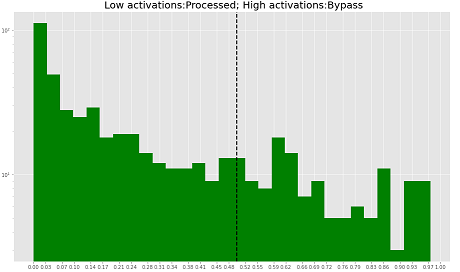
\includegraphics{img_proc_vs_bypass.png}
\caption{Gate unit activations}
\end{figure}

    \hypertarget{cifar-10-results-and-metrics-analysis}{%
\subsection{CIFAR-10 results and metrics
analysis}\label{cifar-10-results-and-metrics-analysis}}

The results of the grid-searching experiment on CIFAR can be inspected
in the below table. The results are also promising, as the \emph{MGU}
based model achieves comparable validation accuracy with the best non
\emph{MGU} model. The running time (\texttt{tts} column) for the
\emph{MGU} based model is 1089 seconds, whereas the basic grid search
runs in approximately 13450 seconds - 12.35x speedup. This result
drastically improves the energy consumption and the carbon footprint.

The model size column - \texttt{model\_sz\ (M)} - is represented in
millions of parameters.

\begin{longtable}[]{@{}rlllrrrrr@{}}
\toprule
& model\_name & layout & norm & residual & model\_sz (M) & tts &
train\_acc & val\_acc\tabularnewline
\midrule
\endhead
0 & CIF\_016 & {[}10, 1, 2, 8, 1.32{]} & bn\_pre & 0 & 2.41 & 494 &
88.72 & 74.38\tabularnewline
1 & CIF\_008 & {[}15, 1, 2, 8, 1.32{]} & bn\_pre & 0 & 30.51 & 1456 &
93.06 & 74.13\tabularnewline
2 & CIF\_MGU\_002 & {[}7, 2, 2, 5, 1.32{]} & N/A & N/A & 3.09 & 1089 &
95.02 & 73.96\tabularnewline
3 & CIF\_006 & {[}15, 1, 2, 8, 1.32{]} & bn\_post & 0 & 30.51 & 910 &
92.71 & 73.83\tabularnewline
4 & CIF\_014 & {[}10, 1, 2, 8, 1.32{]} & bn\_post & 0 & 2.41 & 347 &
92.2 & 73.2\tabularnewline
5 & CIF\_024 & {[}7, 2, 2, 5, 1.32{]} & bn\_pre & 0 & 0.44 & 386 & 87.55
& 71.18\tabularnewline
6 & CIF\_022 & {[}7, 2, 2, 5, 1.32{]} & bn\_post & 0 & 0.44 & 244 &
86.52 & 70.24\tabularnewline
7 & CIF\_011 & {[}10, 1, 2, 8, 1.32{]} & ln & 1 & 4.81 & 689 & 82.37 &
68.96\tabularnewline
8 & CIF\_021 & {[}7, 2, 2, 5, 1.32{]} & bn\_post & 1 & 0.88 & 319 &
81.82 & 68.74\tabularnewline
9 & CIF\_020 & {[}7, 2, 2, 5, 1.32{]} & ln & 0 & 0.44 & 251 & 84.79 &
68.68\tabularnewline
10 & CIF\_018 & {[}7, 2, 2, 5, 1.32{]} & no\_norm & 0 & 0.44 & 235 &
86.51 & 67.78\tabularnewline
11 & CIF\_019 & {[}7, 2, 2, 5, 1.32{]} & ln & 1 & 0.88 & 548 & 91.74 &
67.34\tabularnewline
12 & CIF\_013 & {[}10, 1, 2, 8, 1.32{]} & bn\_post & 1 & 4.81 & 699 &
85.83 & 66.92\tabularnewline
13 & CIF\_015 & {[}10, 1, 2, 8, 1.32{]} & bn\_pre & 1 & 4.81 & 715 &
75.75 & 66.08\tabularnewline
14 & CIF\_023 & {[}7, 2, 2, 5, 1.32{]} & bn\_pre & 1 & 0.88 & 344 & 73 &
65.29\tabularnewline
15 & CIF\_010 & {[}10, 1, 2, 8, 1.32{]} & no\_norm & 0 & 2.4 & 258 &
83.32 & 61.09\tabularnewline
16 & CIF\_017 & {[}7, 2, 2, 5, 1.32{]} & no\_norm & 1 & 0.88 & 270 &
49.24 & 47.91\tabularnewline
17 & CIF\_009 & {[}10, 1, 2, 8, 1.32{]} & no\_norm & 1 & 4.8 & 213 &
47.26 & 44.85\tabularnewline
18 & CIF\_007 & {[}15, 1, 2, 8, 1.32{]} & bn\_pre & 1 & 60.99 & 1579 &
46.4 & 43.47\tabularnewline
19 & CIF\_MGU\_001 & {[}15, 1, 2, 8, 1.32{]} & N/A & N/A & 182.93 & 2115
& 34.98 & 33.95\tabularnewline
20 & CIF\_005 & {[}15, 1, 2, 8, 1.32{]} & bn\_post & 1 & 60.99 & 777 &
26.25 & 25.82\tabularnewline
21 & CIF\_003 & {[}15, 1, 2, 8, 1.32{]} & ln & 1 & 60.98 & 733 & 20.14 &
20.2\tabularnewline
22 & CIF\_001 & {[}15, 1, 2, 8, 1.32{]} & no\_norm & 1 & 60.96 & 1058 &
17.67 & 17.71\tabularnewline
23 & CIF\_002 & {[}15, 1, 2, 8, 1.32{]} & no\_norm & 0 & 30.49 & 366 &
10 & 10\tabularnewline
24 & CIF\_012 & {[}10, 1, 2, 8, 1.32{]} & ln & 0 & 2.41 & 187 & 10 &
10\tabularnewline
25 & CIF\_004 & {[}15, 1, 2, 8, 1.32{]} & ln & 0 & 30.5 & 417 & 10 &
10\tabularnewline
\bottomrule
\end{longtable}

The first \emph{MGU} based model - \emph{CIF\_MGU\_001} that used the 15
stacked computational modules which is the maximum number of
computational modules in the chosen CIFAR-10 grid search. As a result,
this model is over-parametrized and thus, its optimization diverges
after the first epoch. The over-parametrization comes from the added
gate transformations for \emph{Convolutional} layers. We train another
\emph{MGU} based model that uses less computational elements -
\emph{CIF\_MGU\_002} - and it behaves as expected.

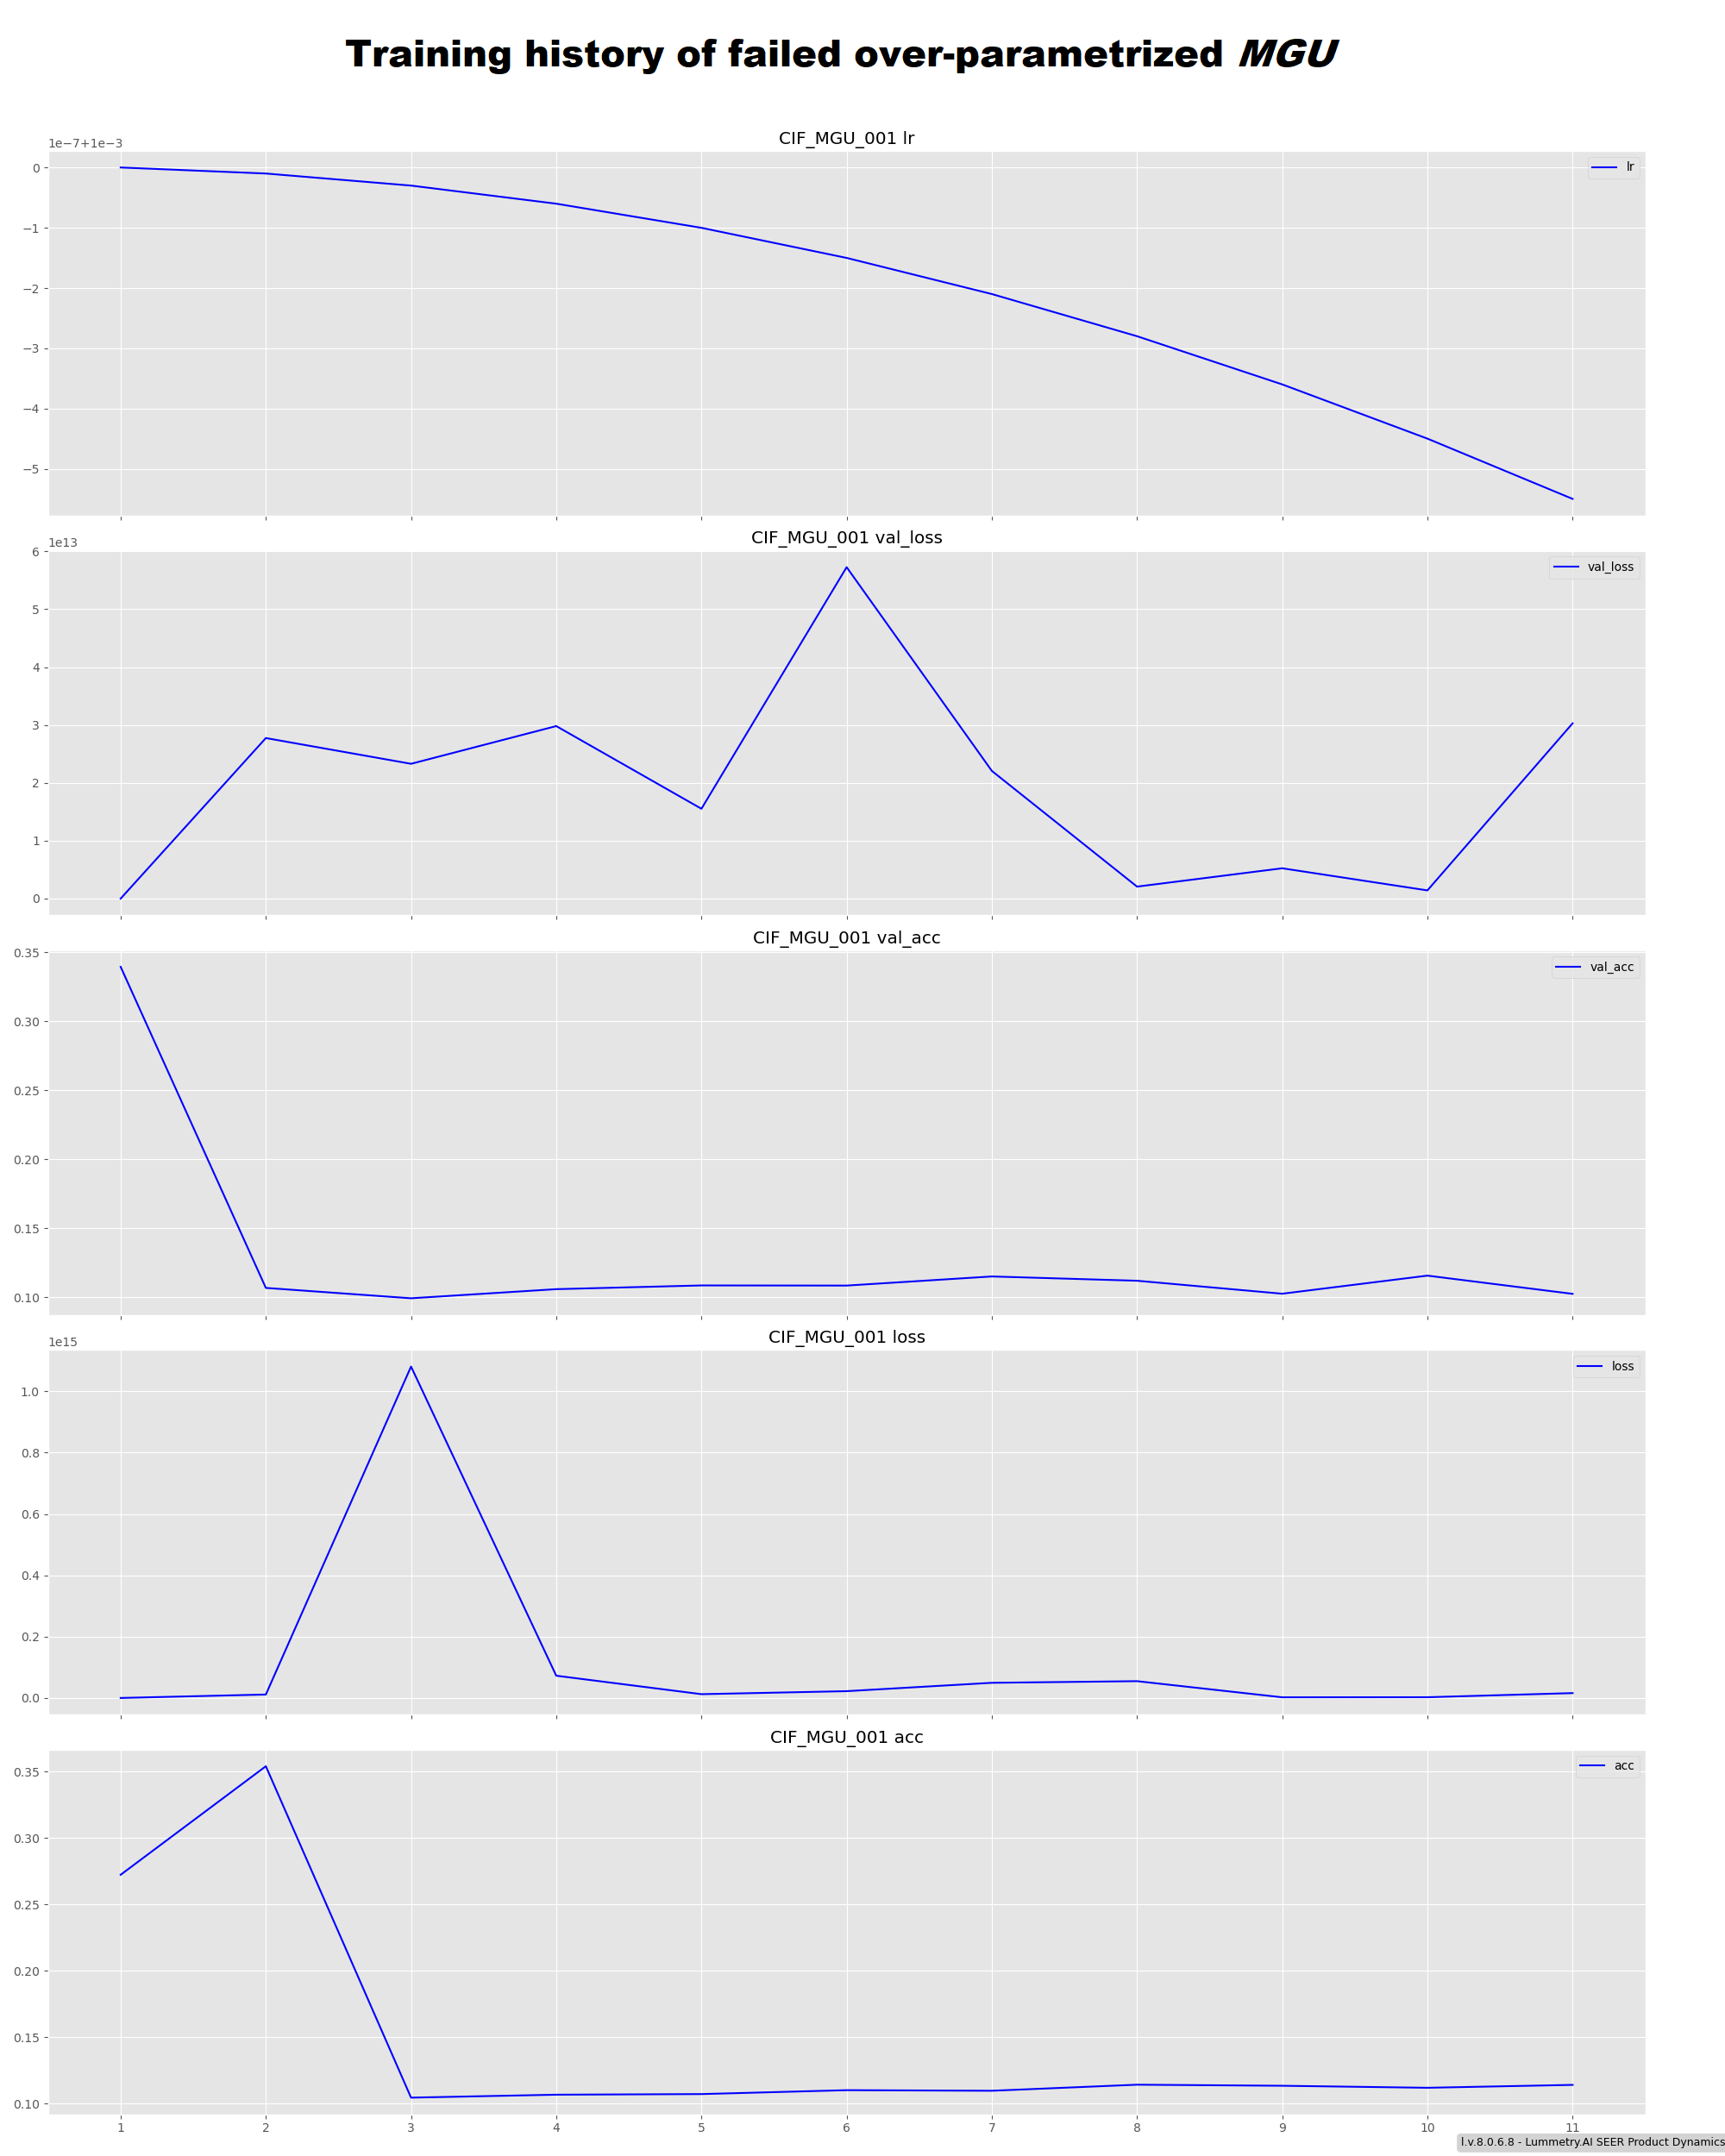
\includegraphics{img_cifar10_mgu_fail.png}

    \hypertarget{the-next-steps}{%
\section{The next steps}\label{the-next-steps}}

So far we managed to obtain a stable version of the \emph{MGU} module
including the self-explanation feature for Tensorflow. We also prepared
a lighter version of \emph{MGU} for PyTorch framework. We also
experimented and evaluated the behavior of the MGU on two initial public
datasets and clearly identified the need to have more efficient gating
transformations. Beside the public dataset experimental work we already
employed the \emph{MGU} on private production-grade systems.

\hypertarget{cervigram-experiment}{%
\subsection{CERVIGRAM experiment}\label{cervigram-experiment}}

More work is required to obtain consistent evidence regarding the
application of our proposed innovation. Currently experimentation is
underway with CERVIGRAM dataset.

\hypertarget{predictive-analytics-experiment}{%
\subsection{Predictive analytics
experiment}\label{predictive-analytics-experiment}}

Moreover, we will prepare for the final paper experiments proof that
\emph{MGU} can be applied to other \emph{layer} types such as
\emph{linear} layers in predictive analytics experiments. The
application of \emph{MGU} on private datasets already has yielded good
results and we are preparing the report on those experiments as well.

\hypertarget{over-parametrization}{%
\subsection{Over-parametrization}\label{over-parametrization}}

Moreover, we will address the over parametrization problem efficiently
either with heuristical approaches such as using depth-wise convolutions
transformations for convolutional gates or with low-dimensionality
embedding generation similar to \cite{hu2019squeezeandexcitation}. Last
but not least we will explore further feature processors possibilities
to include in the \emph{MultiGatedUnit}.

		\begin{Verbatim}[commandchars=\\\{\},fontsize=\scriptsize]
{\color{incolor}In [{\color{incolor} }]:} 
\end{Verbatim}


    % Add a bibliography block to the postdoc
    
    
\bibliographystyle{unsrt}
\bibliography{jupyter}

    
\end{document}
